\RequirePackage{rotating}
\documentclass{article}

% Bibliography
\usepackage{natbib}
\bibpunct{(}{)}{;}{a}{}{;}

% Use 'It was found that A is B (Name 1234)' style
\setcitestyle{authoryear,open={},close={}}

% Affiliations
\usepackage{authblk}
\title{pirouette: Determining the error BEAST2 makes in inferring a phylogeny}
\author[1]{Rich\`el J.C. Bilderbeek}
\author[1]{Giovanni Laudanno}
\author[1]{Rampal S. Etienne}
\affil[1]{Groningen Institute for Evolutionary Life Sciences, University of Groningen, Groningen, The Netherlands}

% Use double spacing
\usepackage{setspace}
\doublespacing

\usepackage{listings}
\usepackage{hyperref}
\usepackage{todonotes}
\usepackage{verbatim}
\usepackage{pgf}
\usepackage{bm}
\usepackage{multirow}
\usepackage{amsfonts}
\usepackage{array}
\usepackage{array}
\usepackage{booktabs}
\newcolumntype{C}[1]{>{\centering\arraybackslash}p{#1}}
\newcolumntype{L}[1]{>{\raggedright\arraybackslash}p{#1}}
\usepackage{longtable}
\usepackage{rotating}
\usepackage{mathtools}

\usepackage{tkz-graph}
\usetikzlibrary{arrows,automata}
\usetikzlibrary{calc}
\usetikzlibrary{arrows.meta}

% sidewaysfigure
\usepackage{rotating}

% Style of listings
% From http://r.789695.n4.nabble.com/How-to-nicely-display-R-code-with-the-LaTeX-package-listings-tp4648110.html
\usepackage{fancyvrb} 
\definecolor{codegreen}{rgb}{0,0.6,0}
\definecolor{codegray}{rgb}{0.5,0.5,0.5}
\definecolor{codepurple}{rgb}{0.58,0,0.82}
\definecolor{backcolor}{rgb}{0.95,0.95,0.92}
\lstdefinestyle{mystyle}{
  language=R,% set programming language
  basicstyle=\ttfamily\small,% basic font style
  commentstyle=\color{gray},% comment style
  % numbers=left,% display line numbers on the left side
  numberstyle=\scriptsize,% use small line numbers
  numbersep=10pt,% space between line numbers and code
  tabsize=2,% sizes of tabs
  showstringspaces=false,% do not replace spaces in strings by a certain character
  captionpos=b,% positioning of the caption below
  breaklines=true,% automatic line breaking
  escapeinside={(*}{*)},% escaping to LaTeX
  fancyvrb=true,% verbatim code is typset by listings
  extendedchars=false,% prohibit extended chars (chars of codes 128--255)
  alsoletter={.<-},% becomes a letter
  alsoother={$},% becomes other
  otherkeywords={!=, ~, $, \&, \%/\%, \%*\%, \%\%, <-, <<-, /},% other keywords
  deletekeywords={c}% remove keywords 
}
\lstset{style=mystyle}

% Adds numbered lines
\usepackage{lineno}
\linenumbers

% Rename 'Abstract' to 'Summary 
\usepackage[english]{babel}
\addto{\captionsenglish}{\renewcommand{\abstractname}{Summary}}

%comments
\newcommand{\giovanni}[1]{\textcolor{blue}{\textbf{[GL: #1]}}}
\newcommand{\richel}[1]{\textcolor{orange}{\textbf{[RB: #1]}}}
\newcommand{\rampal}[1]{\textcolor{green}{\textbf{[RSE: #1]}}}


\begin{document}

\maketitle

\begin{abstract}

  \textbf{1. }
    BEAST2 is a popular Bayesian phylogenetics software tool,
    that takes an alignment of characters (usually nucleotides) 
    and an inference model to create a
    posterior of jointly-estimated phylogenies and model parameter 
    estimates. An important ingredient of BEAST2 is 
    the model for the species tree prior, 
    and the tool can in principle be used for inference of 
    macroevolutionary processes underlying the species tree. 
    However, only models that allow for fast computation of 
    the prior probability are possible in practice. 
    This begs the question of how accurate the tree estimation is 
    when the real macroevolutionary processes are different 
    from those assumed in BEAST2. \\
  \textbf{2. }
    Here we present \verb;pirouette;, 
    a free, libre and open-source R package that assesses 
    the inference error BEAST2 makes based on a known/true 
    phylogeny, for example generated by a new 
    macroevolutionary diversification model. \\
  \textbf{3. }
    We describe \verb;pirouette;'s usage and the biological scientific
    question it can answer, including full examples. \\
  \textbf{4. }
    Last, we discuss the results obtained by the examples. \\
\end{abstract}

{\bf Keywords:} computational biology, evolution, phylogenetics, BEAST2, pirouette, R

%%%%%%%%%%%%%%%%%%%%%%%%%%%%%%%%%%%%%%%%%%%%%%%%%%%%%%%%%%%%%%%%%%%%%%%%%%%%%%%%%%%%%%
\section{Introduction}
%%%%%%%%%%%%%%%%%%%%%%%%%%%%%%%%%%%%%%%%%%%%%%%%%%%%%%%%%%%%%%%%%%%%%%%%%%%%%%%%%%%%%%

The development of new powerful inference tools, 
such as BEAST [\cite{drummond2007beast}], 
MrBayes [\cite{huelsenbeck2001mrbayes}]
or RevBayes [\cite{hohna2016revbayes}], 
allows to build phylogenetic trees 
from character data (usually nucleotide sequences) extracted 
from extant (but also extinct) organisms.
This has constituted an important step forward 
in our understanding of how species evolve.
Such tools have been increasingly exploited to hypothesize 
and test what the main drivers and modes for diversification are.

Because BEAST performs a Bayesian analysis, 
it does not only need character data but also tree priors, 
describing how the diversification occurs, to return posterior phylogenies.
BEAST uses standard tree priors such as Yule or 
constant-rate birth-death [\cite{nee1994reconstructed}] models.
These models are most commonly picked in biological research,
as these are of a desired minimum biological complexity, 
yet computationally fast enough.
The recent development of BEAST2 [\cite{bouckaert2014beast}] provides, 
unlike its predecessor, the possibility for third-party users 
to use their own new or preferred diversification model, 
if an algorithm is provided to calculate the probability 
of a tree given such a diversification model.
There have been plenty of these models (and their associated probability algorithms) 
developed, among others, those in which diversification is 
time-dependent [\cite{nee1994reconstructed}, \cite{rabosky2008explosive}], 
or diversity-dependent [\cite{etienne2011diversity}],
or that can shift [\cite{etienne2012conceptual}, \cite{rabosky2014automatic}, \cite{alfaro2009nine}, the SLS model. Laudanno et al., in preparation].
Other birth-death models treat speciation as a process that takes time [\cite{rosindell2010protracted}][\cite{etienne2012prolonging}], or that happens in bursts of simultaneous events [Laudanno et al., in preparation], or that
depends on a trait that has two [\cite{maddison2007estimating}], 
or more [\cite{fitzjohn2012diversitree}] states,
or even allows concealed states [\cite{beaulieu2016detecting}] 
or a combination of all these [\cite{herrera2018detecting}].
Not all of these diversification models are available in BEAST2, 
but the option is available.

For a given phylogeny, the parameter values of the diversification model 
are usually estimated using maximum likelihood.
For such  models, 
it is a standard practice to assess their performance 
on a controlled environment: 
phylogenies are simulated with known parameters, 
and then the estimated parameters are compared with the original parameters.
If the likelihood proves to be effective to describe the process, 
it can potentially be implemented into BEAST2 as a new prior. 
However, in many cases the computation of this likelihood (the tree prior) 
is computationally demanding and it is unfeasible to use it 
in a Bayesian inference framework where it needs to be 
computed millions to billions of times.
However, if the data are very informative, the influence of the prior 
is often relatively small, and hence under this assumption 
it has become common practice to use already existing BEAST2 priors. 
However, it is unclear whether this assumption holds.
Here we introduce a pipeline to assess this assumption 
for any given diversification model. 
Briefly, it consists of the following steps: 
first simulate a phylogeny 
according to the mechanisms proposed by the new diversification model, 
then simulate a nucleotide alignment 
and use current inference tools (such as BEAST2) to estimate the phylogeny. 
If the estimated tree differs only slightly from the original phylogeny, 
the original assumption is justified and the simple diversification models 
in the inference tools suffice. 
If the trees differ markedly, it will be worth the effort and computational burden 
to develop a species tree module to be used in these tools.
Our pipeline is programmed as an R package and is called 
\verb;pirouette; it is built on \verb;babette; [Bilderbeek \& Etienne, 2018], 
which calls BEAST2 [\cite{bouckaert2014beast}]. 
With \verb;pirouette;, one
can easily measure the error made by Bayesian inference in recovering
any given phylogeny, helping us to evaluate the necessity of a new diversification model.

%%%%%%%%%%%%%%%%%%%%%%%%%%%%%%%%%%%%%%%%%%%%%%%%%%%%%%%%%%%%%%%%%%%%%%%%%%%%%%%%%%%%%%
\section{Description}
%%%%%%%%%%%%%%%%%%%%%%%%%%%%%%%%%%%%%%%%%%%%%%%%%%%%%%%%%%%%%%%%%%%%%%%%%%%%%%%%%%%%%%

\verb;pirouette; is written in the R programming language (\cite{R}).
The goal of \verb;pirouette; is to measure the inference error BEAST2
makes for a given reconstructed phylogeny, 
simulated under the mechanisms of a (possibly new) diversification model, 
which we will refer to as the 'generative prior'. 
Such a study will typically construct phylogenies 
for different combinations of the diversification model's parameters, 
to assess under which scenarios the error made by BEAST2 cannot be neglected. 
Although a well-conducted theoretical study uses many replicates, 
this article only shows examples with one replicate, for the sake of clarity.

\verb;pirouette; is very flexible and allows the user 
to specify a big variety of custom settings. 
These settings can be grouped in macro-sections, 
according to how they operate in the pipeline. 
We summarize them in Tables~\ref{tab:options} and \ref{tab:definitions}.

Although many possible tests can be performed, 
we present here only four \giovanni{five?} example research questions (ERQ) that \verb;pirouette; can answer. 
For these ERQs we will estimate the error made by BEAST2 when 
using a birth-death tree prior, in recovering an original tree 
generated under a Yule generative prior.



\begin{sidewaystable}
\centering
  \begin{tabular}{|@{}c|p{2.5cm}|p{9cm}|p{4.5cm}@{}|}
    \hline
    \centering
    \textbf{Symbol} & \textbf{Sub-argument} & \textbf{Description} & \textbf{Possible values} \\ 
    \hline
    $\mathit{t_{p}}$ & tree prior & Macroevolutionary speciation model & Yule, BD, CBS, CCP, CEP \\
    $\mathit{c_{m}}$ & clock model & Clock for the DNA mutation rates & strict, relaxed log-normal \\
    $\mathit{s_{m}}$ & site model & Nucleotide substitution model & JC, HKY, TN93, GTR \\
    $\mathit{m_{r}}$ & mutation rate & Pace at which mutation occurs & $m_{r} \in \mathbb{R}_{>0}$\\
    $\mathit{r_{s}}$ & root sequence & DNA sequence at the root of the tree & any combination of a, c, g, t \\
    $\mathit{m_{p}}$ & MRCA prior & Prior knowledge of a most recent common ancestor & see documentation \\
    $\mathit{m_{s}}$ & MCMC settings & Markov Chain Monte Carlo algorithm setup & see documentation \\
    $\mathit{m_{t}}$ & model type & Criterion to select an inference model & Generative, Candidate \\
    $\mathit{r_{i}}$ & run if & Condition under which an inference model is used & Always, Best candidate\\
    $\mathit{e_{f}}$ & error function & Specifies how to measure the error & nLTT, $|\gamma|$ \\
    $\mathit{t_{m}}$ & twin model & Sets the tree prior for the twin tree & Yule, BD \\
    \hline
  \end{tabular}
  \caption{
    Most important parameter options. BD = birth death, CBS = coalescent
    Bayesian Skyline, CCP = coalescent constant-population, CEP = coalescent
    exponential-population, JC = Jukes-Cantor 1969 (\cite{jukes1969evolution}), HKY = Hasegawa, Kishino and 
    Yano (\cite{hasegawa1985dating}), TN93 = \cite{tamura1993estimation}, GTR = Generalised time-reversible 
    model (\cite{tavare1986some}).
  }
  \label{tab:options}
\bigskip

  \begin{tabular}{|@{}c|p{4cm}|p{9cm}|p{3cm}@{}|}
    \hline
    \centering
    \textbf{Symbol} & \textbf{Macro-argument} & \textbf{Description} & \textbf{Includes} \\
    \hline
    $\mathit{G}$ & Generative prior & Diversification model to generate the 'true' tree & $\mathit{t_{p}}$ \\
    $\mathit{A}$ & Alignment model & Model used to simulate the alignment ($\mathit{c_{m}}$ must be strict) & $\mathit{c_{m}}, \mathit{s_{m}}, \mathit{m_{r}}, \mathit{r_{s}}$ \\
    $\mathit{I}$ & Inference model & Phylogenetic inference model to run BEAST2 & $\mathit{c_{m}},\mathit{s_{m}},\mathit{t_{p}},\mathit{m_{p}},\mathit{m_{s}}$ \\
    $\mathit{C}$ & Inference conditions & Conditions under which $\mathit{I}$ is used in the inference & $\mathit{m_{t}}, \mathit{r_{i}}$\\
    $\mathit{X}$ & Experiment & Full setting for the BEAST2 run & $\mathit{I},\mathit{C}$ \\
    $\mathit{E}$ & Error measure parameters & Errors measurement setup & $\mathit{e_{f}}$\\
    $\mathit{T}$ & Twinning parameters & Twin tree creation procedure & $\mathit{t_{m}}$\\
    \hline 
  \end{tabular}
  \caption{
    Definitions of terms and relative symbols used in the main text and in Fig~\ref{fig:pipeline}.
  }
  \label{tab:definitions}
  \giovanni{Should we rename "Twinning Parameters" to "Twinning model" and "twin model" to "twin prior"?}
\end{sidewaystable}

\iffalse
\begin{table}
\centering
  \begin{tabular}{|@{}c|p{2.8cm}|p{6cm}@{}|}
    \hline
    \textbf{Symbol} & \textbf{Name} & \textbf{Definition} \\ 
    \hline
    $\mathit{t}$ & Tree prior & Macroevolutionary speciation model \\
    $\mathit{c}$ & Clock model & Clock for the DNA mutation rates\\
    $\mathit{s}$ & Site model & Nucleotide substitution model\\
    $\mathit{\mu}$ & Mutation rate & Pace at which mutation occurs, $\mu \in \mathit{s}$ \\
    $\mathit{r}$ & Root sequence & DNA sequence at the root of the tree\\
    $\mathit{m}$ & MRCA prior & Prior knowledge of a most recent common ancestor \\
    $\mathit{v}$ & MCMC settings & Markov Chain Monte Carlo algorithm setup \\
    \hline
    $\mathit{P}$ & Generative prior & Diversification model under which the 'true' tree is simulated \\
    $\mathit{A}$ & Alignment model & Alignment simulation model. It is a combination of $(\mathit{r}, \mathit{\mu}, \mathit{c}, \mathit{s})$, where $\mathit{c}$ = strict \\
    $\mathit{G}$ & Generative model & Combination of a known $\mathit{P}$ and chosen (thus known) $\mathit{A}$ \\
    $\mathit{I}$ & Inference model & Bayesian phylogenetic inference model, a combination of
    $(\mathit{c},\mathit{s},\mathit{t},\mathit{m},\mathit{v})$\\
    $\mathit{C}$ & Inference conditions & Conditions under which $\mathit{I}$ is used in the inference \\
    $\mathit{X}$ & Experiment & Combination of $(\mathit{I},\mathit{C})$\\
    $\mathit{E}$ & Error measurement parameters & Errors measurement setup \\
    $\mathit{T}$ & Twinning parameters & Twin tree creation procedure \\
    \hline 
  \end{tabular}
  \caption{
    Definitions of terms and relative symbols used in this article.
  }
  \label{tab:definitions}
  \richel{I've some set notations in some spots, as I am unsure if you like it}
  \giovanni{It would be nice to specify (in the first part of the table) 
    the basic elements composing all the elements of the second part of the table. 
    This could be probably done for "Alignment parameters", "Inference conditions" 
    and "Twinning parameters".
  }
  \richel{
    I feel the next table (which was also your suggestion), does so
    at the right amount of detail
  }
  \giovanni{
    How do we specify what constitutes 'twinning parameters'?
  }
  \richel{Perhaps you'd enjoy my definition?}
\end{table}
\fi

\iffalse
% previous version
\begin{table}
\centering
  \begin{tabular}{|@{}c|p{2.8cm}|@{}l|p{5.5cm}@{}|}
    \hline
    \textbf{Symbol} & \textbf{Name} & \textbf{Definition} \\ 
    \hline
    $\mathit{t}$ & Tree prior & Macroevolutionary speciation model \\
    $\mathit{c}$ & Clock model & Clock for the DNA mutation rates\\
    $\mathit{s}$ & Site model & Nucleotide substitution model\\
    $\mathit{\mu}$ & Mutation rate & Pace at which mutation occurs, $\mu \in \mathit{s}$ \\
    $\mathit{r}$ & Root sequence & DNA sequence at the root of the tree\\
    $\mathit{m}$ & MRCA prior & Prior knowledge of a most recent common ancestor\\
    $\mathit{v}$ & MCMC settings & Markov Chain Monte Carlo algorithm setup \\
    \hline
    $\mathit{G}$ & Generative prior & Diversification model the 'true' tree is simulated with \\
    $\mathit{A}$ & Alignment model & Alignment simulation model, $\mathit{A} \ni \{ \mathit{r}, \mathit{\mu}, \mathit{c}, \mathit{s} \}$, in which $\mathit{c}$ = strict \\
    $\mathit{G}$ & Generative model & Combination of a known $\mathit{P}$ and chosen (thus known) $\mathit{A}$ \\
    $\mathit{I}$ & Inference model & Bayesian phylogenetic inference model, a combination of
    $(\mathit{c},\mathit{s},\mathit{t},\mathit{m},\mathit{v})$\\
    $\mathit{C}$ & Inference conditions & Conditions under which $\mathit{I}$ is used in inference \\
    $\mathit{X}$ & Experiment & Combination of $(\mathit{I},\mathit{C})$\\
    $\mathit{E}$ & Error measurement parameters & Errors measurement setup \\
    $\mathit{T}$ & Twinning parameters & Twin tree creation procedure \\
    \hline 
  \end{tabular}
  \caption{
    Definitions of terms and relative symbols used in this article.
  }
  \label{tab:definitions}
  \richel{I've some set notations in some spots, as I am unsure if you like it}
  \giovanni{It would be nice to specify (in the first part of the table) 
    the basic elements composing all the elements of the second part of the table. 
    This could be probably done for "Alignment parameters", "Inference conditions" 
    and "Twinning parameters".
  }
  \richel{
    I feel the next table (which was also your suggestion), does so
    at the right amount of detail
  }
  \giovanni{
    How do we specify what constitutes 'twinning parameters'?
  }
  \richel{Perhaps you'd enjoy my definition?}
\end{table}
\fi

\iffalse
% previous version
\begin{table}
\centering
  \begin{tabular}{| c | c | l |}
    \hline
    \textbf{Symbol} & \textbf{Subparameter} & \textbf{Possible values} \\ 
    \hline
    $\mathit{t}$ & name & Yule, BD, CBS, CCP, CEP \\
    $\mathit{c}$ & clock model & strict, relaxed log-normal \\
    $\mathit{s}$ & site model & JC, HKY, TN, GTR \\
    $\mathit{C}$ & model type & Generative, candidate \\
    $\mathit{C}$ & run if & Always, best candidate \\
    $\mathit{E}$ & function & nLTT, $|\gamma|$ \\
    $\mathit{T}$ & model & Yule, BD \\
    \hline
  \end{tabular}
  \caption{
    Most important parameter options. BD = birth death, CBS = coalescent
    Bayesian Skyline, CCP = coalescent constant-population, CEP = coalescent
    exponential-population, JC = Jukes-Cantor 1969, HKY = Hasegawa, Kishino and 
    Yano 1985, TN = Tamura 1992, GTR = Generalised time-reversible 
    model (Tavaré 1986)
  }
  \label{tab:options}
\end{table}
\fi

\subsection{pirouette's pipeline}

\begin{figure}
  \centering
  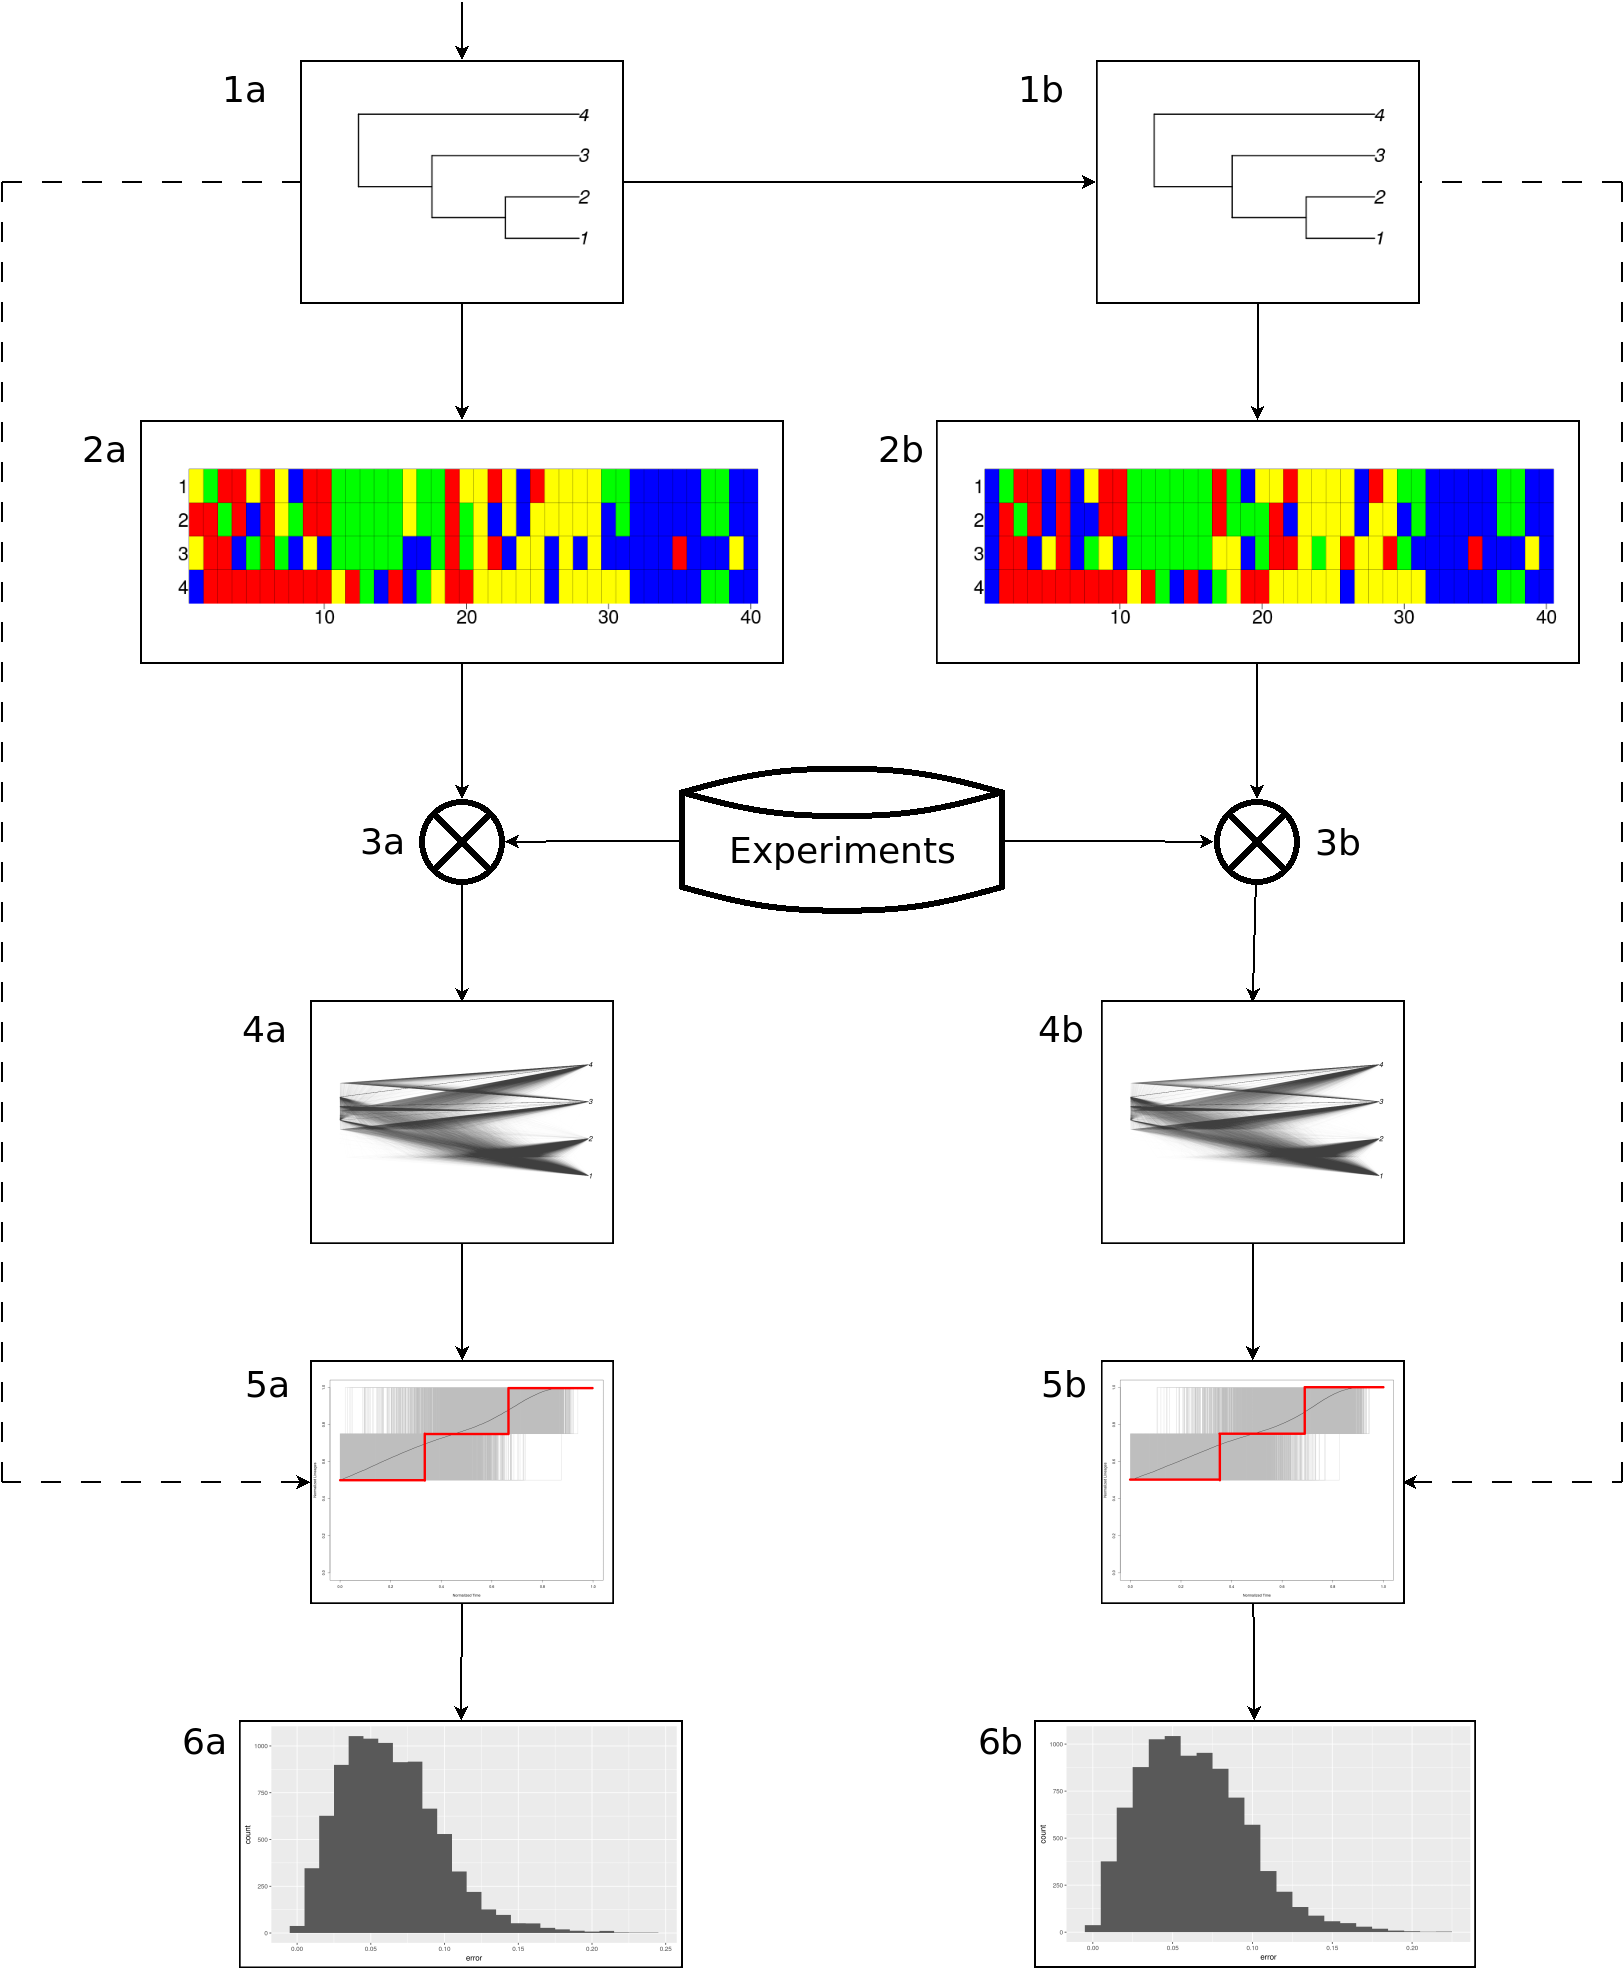
\includegraphics[width=\textwidth]{workflow.png}
  \caption{
    \texttt{pirouette} pipeline. 
    The pipeline starts from a true phylogeny (1a) simulated under the selected generative prior $\mathit{P}$, that is converted to an alignment (2a) according to the alignment model $\mathit{A}$. The user supplies one or more experiments. Every experiment $\mathit{X}$ is defined as a combination of an inference model $\mathit{I}$ and the conditions $\mathit{C}$ under which it is actually used in the inference. Based on the experiments and possibly the alignment (2a), experiments are selected to be actually used in the next step (3a).
    Selected experiments use the alignment (2a) and their inference model $\mathit{I}$ to create a BEAST2 posterior of (parameter estimates and) phylogenies (4a). The posterior trees are compared to the true phylogeny (1a) using the selected error measure $\mathit{E}$, in our case the nLTT statistic [\cite{janzen2015approximate}]. Taking the differences between the true tree's nLTT and each posterior's nLTT results in an error distribution, here displayed as a histogram
    of error values (5a). Optionally, a twin phylogeny (1b) can be generated from the true phylogeny (1a), which then results in an error distribution (5b) with similar intermediate steps.
  }
  \label{fig:pipeline}
  \giovanni{add reference to the generative prior P (or G) in the figure}
  \giovanni{I think that a list of possible models should replace the "experiment" cake in the middle, then C should be drawn on the arrow connecting the figure in the middle to 3a. "I" should replace the circled x of passage 3a. An additional C can be drawn alongside the arrow 2a -> 3a. After that a rectangle can be drawn around the whole middle section (including 3a, 3b and the middle C) to denote that this is phase "X".}
  \giovanni{We might also need an arrow going from the central figure to the top arrow (the one with "T") to specify that the twin is generated according to the chosen inference model.}
\end{figure}

The pipeline is summarized by the following steps, which will be described in detail below:
\begin{enumerate}
    \item for a given phylogeny an alignment is simulated under a known alignment model;
    \item for this alignment, according to the specified inference conditions, an inference model is picked (which may be different from the generative alignment model);
    \item the alignment is then used as BEAST2 input to infer a posterior distribution of phylogenies;
    \item posterior phylogenies are compared with the given original phylogeny to estimate the error made, according to the error measure specified by the user;
\end{enumerate}
The pipeline is visualized in Fig.~\ref{fig:pipeline}. 
There is also the option to generate a 'twin tree', 
that goes through the same pipeline. 
The utility of this twin tree will be explained below.

The first step simulates a DNA alignment from a given 
phylogeny (Fig.~\ref{fig:pipeline}, 1a $\rightarrow$ 2a).
This operation is performed according to the alignment model 
specified by the user, which consists in a root DNA sequence, 
a DNA mutation rate and a site model.
A strict clock model is used as the only clock model
type, as the currently used alignment simulation algorithm
only supports a mutation rate that is equal across all the branches.
This step is relatively fast, 
but longer DNA alignments will noticeably slow down the inference step.

The second step (Fig.~\ref{fig:pipeline}, 2a $\rightarrow$ 3a)
starts from experiments as set up by the user. 
We define an experiment as the combination of an inference model 
and the conditions to actually use it in the inference step.
The inference model can be selected in two ways, either using the
generative model or selecting one or more candidates out of a list of candidate inference models.
An experiment can use the generative model as the inference model, if the generative model is known.
An experiment uses a candidate model if either the generative model is unknown,
or there is an interest in seeing how well non-generative models compete with
the generative model.
Typically, a generative model and/or a best candidate model are used in the actual inference.
When using an experiment with a generative model,
it must use the same site and clock model used in the alignment simulation,
as well as the tree prior that underlied the creation of the given phylogeny. 
When using experiments with candidate models,
\verb;pirouette; selects the best candidate based
on the evidence (i.e. marginal likelihood) for the model given the alignment.
The evidence of an inference model is estimated using a nested sampling (NS)
approach, as described in \cite{maturana2018model}. The nested sampling is
performed by \verb;mcbette; [\cite{mcbette}], that calls the 'NS' BEAST2 package. 
Using BEAST2 packages (in a scripted way) can only be done under Linux and Mac,
therefore the selection of candidate models is not available directly on Windows. 
However, even on Windows systems there is the option to perform the model selection from browser, using \verb;mcbette;, yet the computation for this model selection is
restricted to one hour for free users of the host (Travis CI) continuous
integration service.

The third step infers the actual Bayesian posteriors from the simulated 
alignment (Fig.~\ref{fig:pipeline}, 2a $\rightarrow$ 3a $\rightarrow$ 4a),
using the inference models from the experiments selected in the previous step. For each selected experiment, one BEAST2 posterior is inferred, using the \verb;babette; [\cite{bilderbeek2018babette}] R package.

The fourth step compares the true tree to each posterior tree, resulting in an error distribution (Fig.~\ref{fig:pipeline}, 4a $\rightarrow$ 5a).
The nLTT statistic (\cite{janzen2015approximate}) is used by default, but also a user-defined error statistic can be used. 
As an example, \verb;pirouette; supplies one custom error statistic,
that uses an absolute difference in the gamma statistic [\cite{pybus2000testing}].
Additionally, the user can specify the proportion of posterior phylogenies to 
discard (i.e. the burn-in), throwing away the first $10\%$
of all phylogenies by default. This burn-in is used to discard
the part of the MCMC chain that has not yet converged to a
representative part of the state space.

\subsection{Twin tree}

\iffalse
%version 1
An optional step is to generate a 'twin tree' 
(Fig.~\ref{fig:pipeline}, 1a $\rightarrow$ 1b),
that will be analyzed in the same way as the true tree.
The twin tree will be the true tree 
converted to follow the tree prior of the chosen inference model.

To do so we exploit the likelihood function associated with the chosen inference model. We find the parameters (e.g. speciation and extinction rate for a birth-death model) that maximize such likelihood applied to the true tree, conditioned on its number of tips.

We use these parameters to simulate the branching times of the twin tree, 
which we combine with the original tree's topology.

Using a twin tree serves as a control: both the given/true tree
and twin tree will produce an error distribution.
For the true tree, this error distribution is caused by
the shape of the phylogeny (which is different from the tree priors used), 
the stochastic alignment simulation and stochastic Bayesian inference.  
The twin tree is created from the given phylogeny,
as it has the same topology, 
yet its branching times are simulated according to 
the (implemented) generative tree prior.
Due to this, this error distribution for the twin tree is caused 
only by the stochastic alignment simulation and stochastic Bayesian inference.
The difference between these two error distribution is the error caused
by the new/unimplemented tree prior.
\fi

\iffalse
%version 2 with no formulae
An optional step is to generate a 'twin tree' 
(Fig.~\ref{fig:pipeline}, 1a $\rightarrow$ 1b),
that will be analyzed in the same way as the true tree. We want to produce such tree 'converting' the original tree, created according to the generative prior $\mathit{G}$, into the chosen inference model $\mathit{I}$.

To do so we exploit the likelihood function associated with the chosen inference model $\mathit{I}$. We find the parameters (e.g. speciation and extinction rate for a birth-death model) that maximize such likelihood applied to the true tree, conditioned on its number of tips.

We use these parameters to simulate an equal amount of branching times for the twin tree simulated under the chosen inference model's process. We then combine these branching times with the original tree's topology.

Using a twin tree serves as a control: both the given/true tree and twin tree will produce an error distribution. We assume that these errors are a natural product of the input tree and the intermediate steps of the pipeline. All the factors that can cause such errors are: the branching times of the tree (as a consequence of the tree prior), the topology of the tree, the stochasticity induced by simulating the alignment (step 1a $\rightarrow$ 2a in Fig.~\ref{fig:pipeline}) and the stochasticity induced by the Bayesian inference (step 2a $\rightarrow$ 4a in Fig.~\ref{fig:pipeline}). By imposing the same topology and replicating the pipeline a sufficient number of times we can sort out all the possible causes that are not a direct consequence of the choice of the tree prior.

Potential differences in shapes of error distributions will therefore be consequences of different tree priors for the two parallel pipelines: the use of prior $\mathit{G}$ for the original pipeline and of prior $\mathit{I}$ for the twin pipeline. In the second case, though, such error distribution is not influenced by the mismatch between how the tree is generated and how it is analyzed by BEAST2.
\fi

\giovanni{This is a slightly more formal version. I personally find it clearer. If you don't like it we can use version 2 (see above in the source). In case you really like it, instead, I can try to make the rest a bit more similar to this.}

%version 3, more formal
An optional step is to generate a 'twin tree' $\tau_{I}$
(Fig.~\ref{fig:pipeline}, 1a $\rightarrow$ 1b),
that will be analyzed in the same way as the true tree, following a parallel pipeline. We want to produce such tree 'converting' the original tree $\tau_{G}$, created according to the generative prior $\mathit{G}$, to be in accordance with the chosen inference model $\mathit{I}$:
\begin{align}
    \tau_{G} = (\Vec{t}_{G}, \psi_{G}) \xrightarrow[]{\mathit{T}} \tau_{I} = (\Vec{t}_{I}, \psi_{I}),
\end{align}
where $\Vec{t}$ are the tree branching times and $\psi$ is tree topology, which provides information on where new lineages branch out at each branching time.

To execute the twinning process we exploit the likelihood function $L_{I}$ associated with the chosen inference model $\mathit{I}$. We find the parameters $\theta^{*}_{I}$ (e.g. speciation and extinction rates, in case of a birth-death model) that maximize $L_{I}$ applied to the true tree, conditioned on its number of tips $n_{G}$,
\begin{align}
    max[L_{I}(\theta_{I}|\tau_{G}, n_{G})] \rightarrow \theta^{*}_{I}.
\end{align}
We use $\theta^{*}_{I}$ to simulate an equal amount $n_{I} = n_{G}$ of branching times $\Vec{t}_{I}$ for the twin tree $\tau_{I}$, under the process $I$. We then impose that $\tau_{G}$ and $\tau_{I}$ must respect the same topology
\begin{align}
    \psi_{I} = \psi_{G}.
\end{align}
Using a twin tree serves as a control: both $\tau_{G}$ and $\tau_{I}$ will produce an error distribution. We assume that these errors are a natural product of the input tree and the intermediate steps of the pipeline. All the factors that can cause such errors are: the branching times $\vec{t}$ of the tree (as a consequence of the tree prior), its topology $\psi$, the stochasticity induced by simulating the alignment (step 1a $\rightarrow$ 2a in Fig.~\ref{fig:pipeline}) and the stochasticity induced by the Bayesian inference (step 2a $\rightarrow$ 4a in Fig.~\ref{fig:pipeline}). By imposing the same topology and replicating the pipelines a sufficient number of times we can sort out all the possible causes that are not a direct consequence of the choice of the tree prior.

Potential differences in shape of error distributions will therefore be consequences of different tree priors for the two parallel pipelines: the use of prior $\mathit{G}$ for the original pipeline and of prior $\mathit{I}$ for the twin pipeline. In the second case, though, such error distribution is not influenced by the mismatch between how the tree is generated and how it is analyzed by BEAST2.
%%%%%%%%%%%%%%%%%%%%%%%%%%%%%%%%%%%%%%%%%%%%%%%%%%%%%%%%%%%%%%%%%%%%%%%%%%%%%%%%%%%%%%
\section{Installation}
%%%%%%%%%%%%%%%%%%%%%%%%%%%%%%%%%%%%%%%%%%%%%%%%%%%%%%%%%%%%%%%%%%%%%%%%%%%%%%%%%%%%%%

\verb;pirouette; can be installed easily from CRAN:
\begin{lstlisting}[language=R, floatplacement=ht, frame=single]
install.packages("pirouette")
\end{lstlisting}

For the most up-to-date version, 
one can download and install the package from \verb;pirouette;'s GitHub repository:

\begin{lstlisting}[language=R, floatplacement=ht, frame=single]
usethis::install_github("richelbilderbeek/pirouette")
\end{lstlisting}

To start using \verb;pirouette;, load its functions in the global namespace first:

\begin{lstlisting}[language=R, floatplacement=ht, frame=single]
library(pirouette)
\end{lstlisting}
Because \verb;pirouette; calls BEAST2, BEAST2 must be installed. 
This can be done from within R, using:

\begin{lstlisting}[language=R, floatplacement=ht, frame=single]
install_beast2()
\end{lstlisting}
For the option to select inference models,
\verb;pirouette; uses the "NS" BEAST2 package [\cite{maturana2018model}].
It can be installed from within R, using:

\begin{lstlisting}[language=R, floatplacement=ht, frame=single]
install_beast2_pkg("NS")
\end{lstlisting}

An overview of \verb;pirouette;'s main functions is shown in 
table \ref{tab:functions}. 
We will exploit these functions to answer our research questions in the next sections.

%%%%%%%%%%%%%%%%%%%%%%%%%%%%%%%%%%%%%%%%%%%%%%%%%%%%%%%%%%%%%%%%%%%%%%%%%%%%%%%%%%%%%%
\begin{table}[h]
\centering
\begin{tabular}{ | l | l | }
\hline
\textbf{Name} & \textbf{Description} \\
\hline
\verb;pir_run; & Run \verb;pirouette; \\
\verb;create_pir_params; & Create the \verb;pirouette; parameters \\
\hline
\verb;create_alignment_params; & Create the alignment parameters \\
\verb;create_twinning_params; & Create the twinning parameters \\
\verb;create_experiment; & Create one experiment \\
\verb;create_error_measure_params; & Create the error measurement parameters \\
\hline
\end{tabular}
\caption{pirouette's main functions.}
\label{tab:functions}
\end{table}
%%%%%%%%%%%%%%%%%%%%%%%%%%%%%%%%%%%%%%%%%%%%%%%%%%%%%%%%%%%%%%%%%%%%%%%%%%%%%%%%%%%%%%

All \verb;pirouette;'s functions are documented. 
Useful examples and sensible defaults, 
which we will refer to in the next sections, 
can be accessed from the documentation.

%%%%%%%%%%%%%%%%%%%%%%%%%%%%%%%%%%%%%%%%%%%%%%%%%%%%%%%%%%%%%%%%%%%%%%%%%%%%%%%%%%%%%%
\section{Usage: Example Research Question 1}
%%%%%%%%%%%%%%%%%%%%%%%%%%%%%%%%%%%%%%%%%%%%%%%%%%%%%%%%%%%%%%%%%%%%%%%%%%%%%%%%%%%%%%

A first research question that \verb;pirouette; can answer is:

"What is the error made by BEAST2 from a phylogeny 
using the same diversification model as it was generated by?"

We start from a tree simulated under a Yule (pure-birth) generative prior. 
We choose to use a tree with six taxa and a crown age of ten.

\begin{lstlisting}[
    language=R, floatplacement=ht, frame=single, 
    label = {lst:create_yule_tree}, 
    caption = {
      Create a Yule tree. 
      The resulting tree is shown in figure \ref{fig:yule_tree}
    }
  ]
phylogeny <- create_yule_tree(n_taxa = 6, crown_age = 10)
\end{lstlisting}

\begin{figure}[ht]
  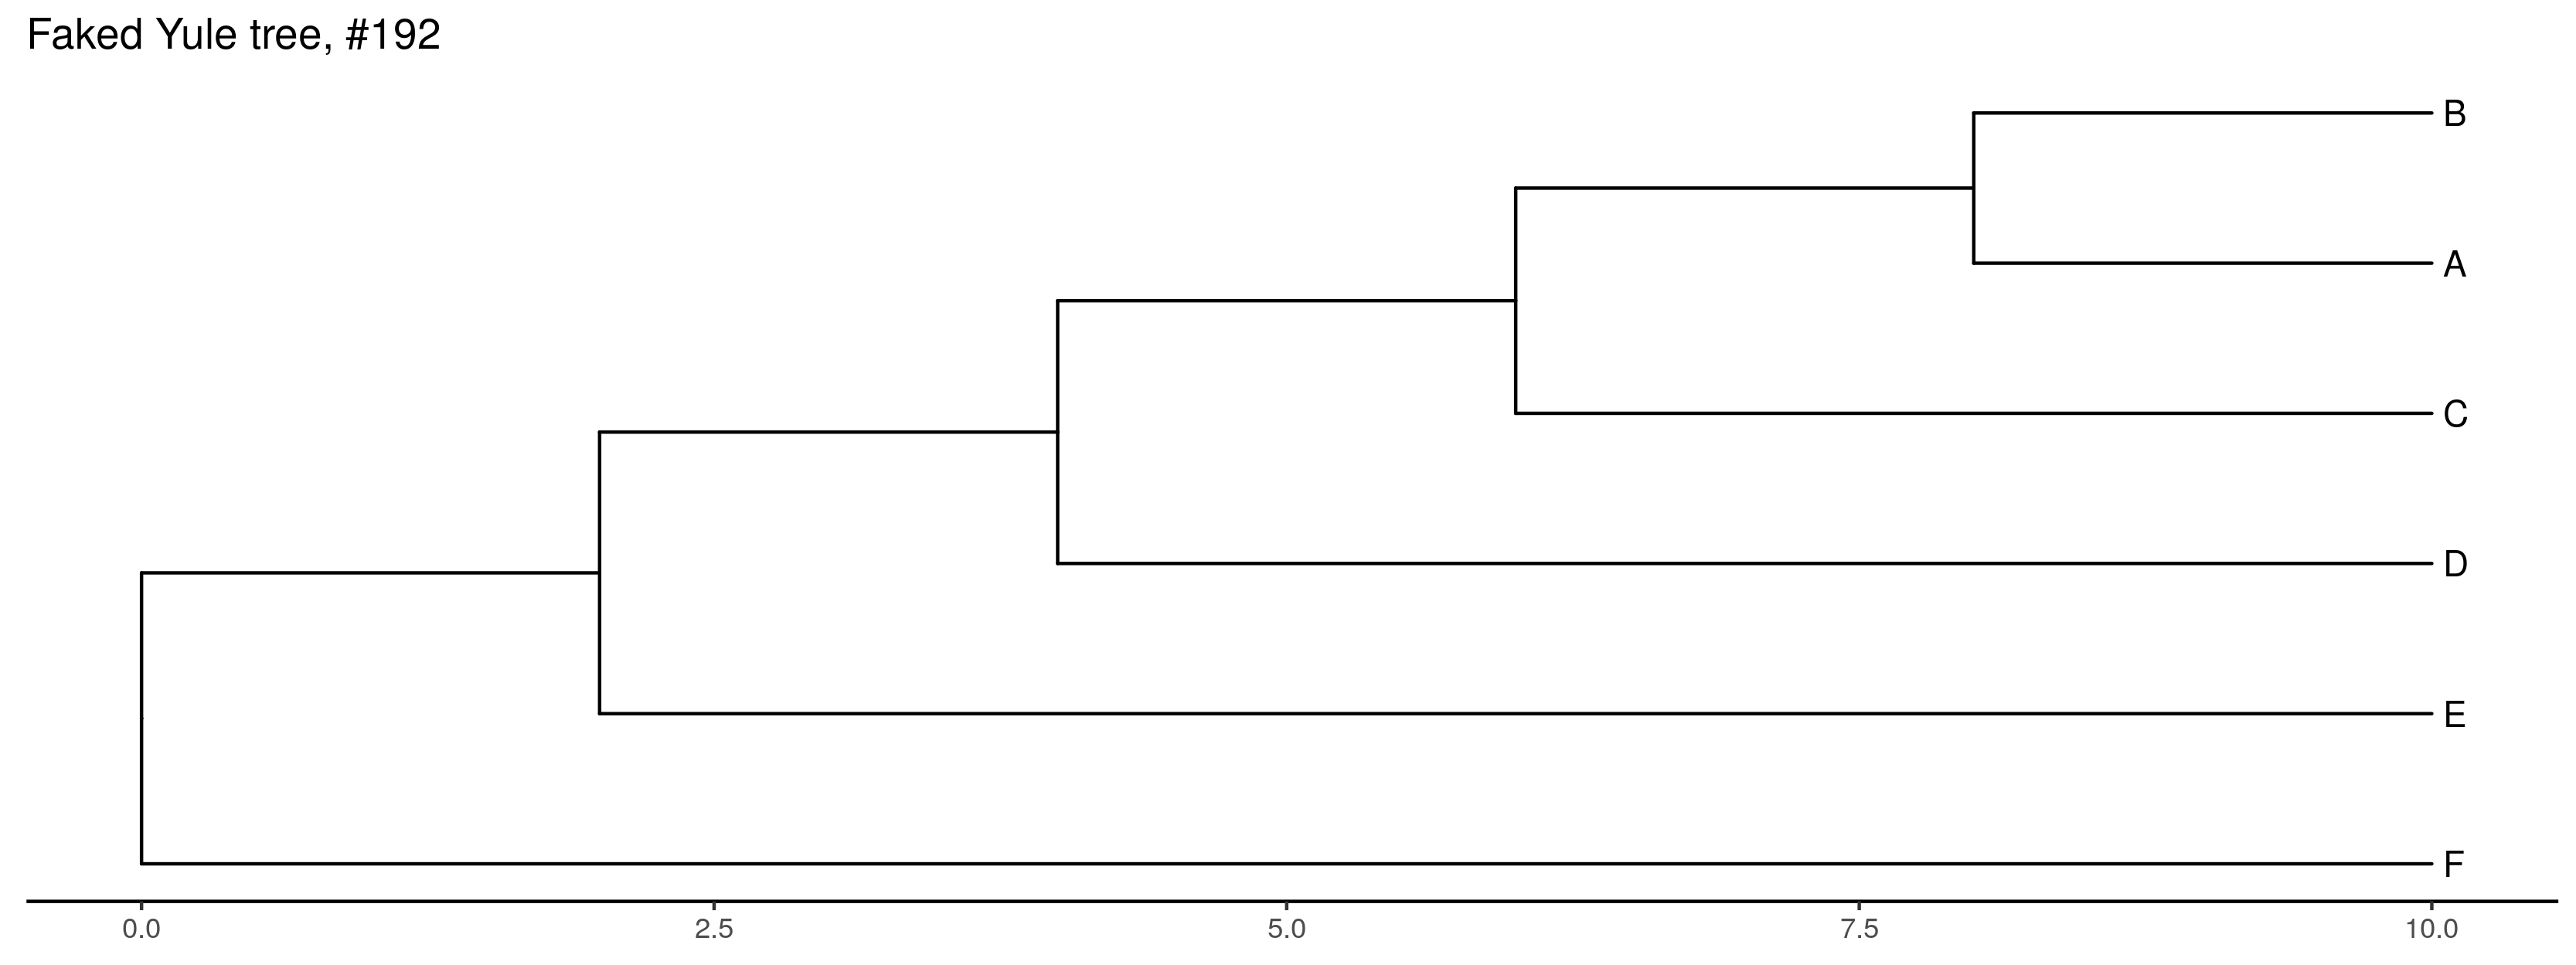
\includegraphics[width=\textwidth]{tree_yule.png}
  \caption{The Yule tree, as created by listing \ref{lst:create_yule_tree}.}
  \label{fig:yule_tree}
  \giovanni{Remove the text in top-left corner.}
  \giovanni{I'd use a sexier topology, purely for esthetical reasons.}
\end{figure}

The first step in \verb;pirouette; is to simulate a DNA alignment from the given phylogeny. 
To do so, we must specify the DNA root sequence and a mutation rate. 
In this example, the DNA root sequence consists in four blocks of 250 nucleotides each, 
where the per-nucleotide mutation rate is 0.1 mutations per unit time.

\begin{lstlisting}[
    language=R,
    floatplacement=ht, frame=single,
    label = {lst:create_alignment}, 
    caption = {Create an alignment.}
  ]
alignment_params <- create_alignment_params(
  root_sequence = create_blocked_dna(length = 1000),
  mutation_rate = 0.1
)
\end{lstlisting}

By default, an alignment is created using a Jukes-Cantor (JC, \cite{jukes1969evolution}) site model
and a strict clock model. 
A JC site model assumes that mutation rates from any nucleotide to any other 
are equal and constant. 
A strict clock model assumes that the mutation rates of all species are equal and constant.
Due to this, we state that the generative model for the alignment is
a JC site model and a strict clock model.

In the second step we state our experiments. In this context, we
define an experiment as a combination of an inference model
and the conditions under which a Bayesian inference is executed.
Within this example, we specify that our experiment uses the
generative model (which means that the inference model will be 
a combination of JC site model, strict clock model and Yule tree prior), 
it will always be run and we skip the evidence measurement for our model.

\begin{table}
  \begin{tabular}{ | c | c | c | l | }
    \hline
    \textbf{model type} & \textbf{run if} & \textbf{measure evidence} & \textbf{inference model} \\ 
    \hline
    generative & always & no & JC, strict, Yule \\
    \hline
  \end{tabular}
  \caption{
    Experimental setup to answer the first research question.
    JC: Jukes-Cantor site model.
    strict: strict clock model.
    Yule: Yule (pure-birth) tree prior.
  }
  \label{tbl:RQ1}
\end{table}

Due to sensible defaults, specifying this
results in:
\giovanni{Would it be clearer not to use sensible defaults where we call the functions with arguments we refer to in the main text? For example here it could be clearer for the reader to see:
create\_experiment(site\_model = create\_jc69\_site\_model(), clock\_model = create\_strict\_clock\_model(), tree\_prior = create\_yule\_tree\_prior())
}

\begin{lstlisting}[
  language=R, 
  floatplacement=ht, frame=single,
  label = {lst:create_generative_experiment},
  caption = {
    Create a default experiment, as described in Table~\ref{tbl:RQ1}.
  }
]
experiments <- list(create_experiment())
\end{lstlisting}

All the \verb;pirouette; arguments are bundled
and checked by \verb;create_pir_params;:

\begin{lstlisting}[language=R, floatplacement=ht, frame=single]
pir_params <- create_pir_params(
  alignment_params = alignment_params,
  experiments = experiments
)
\end{lstlisting}

Running the experiment:

\begin{lstlisting}[language=R, floatplacement=ht, frame=single]
errors <- pir_run(
  phylogeny,
  pir_params = pir_params
)
\end{lstlisting}

\verb;pirouette; has a plotting function used for convenience:

\begin{lstlisting}[language=R, floatplacement=ht, frame=single]
pir_plot(errors)
\end{lstlisting}

The resulting figure is shown in figure \ref{fig:example_1}.

\begin{figure}[ht]
  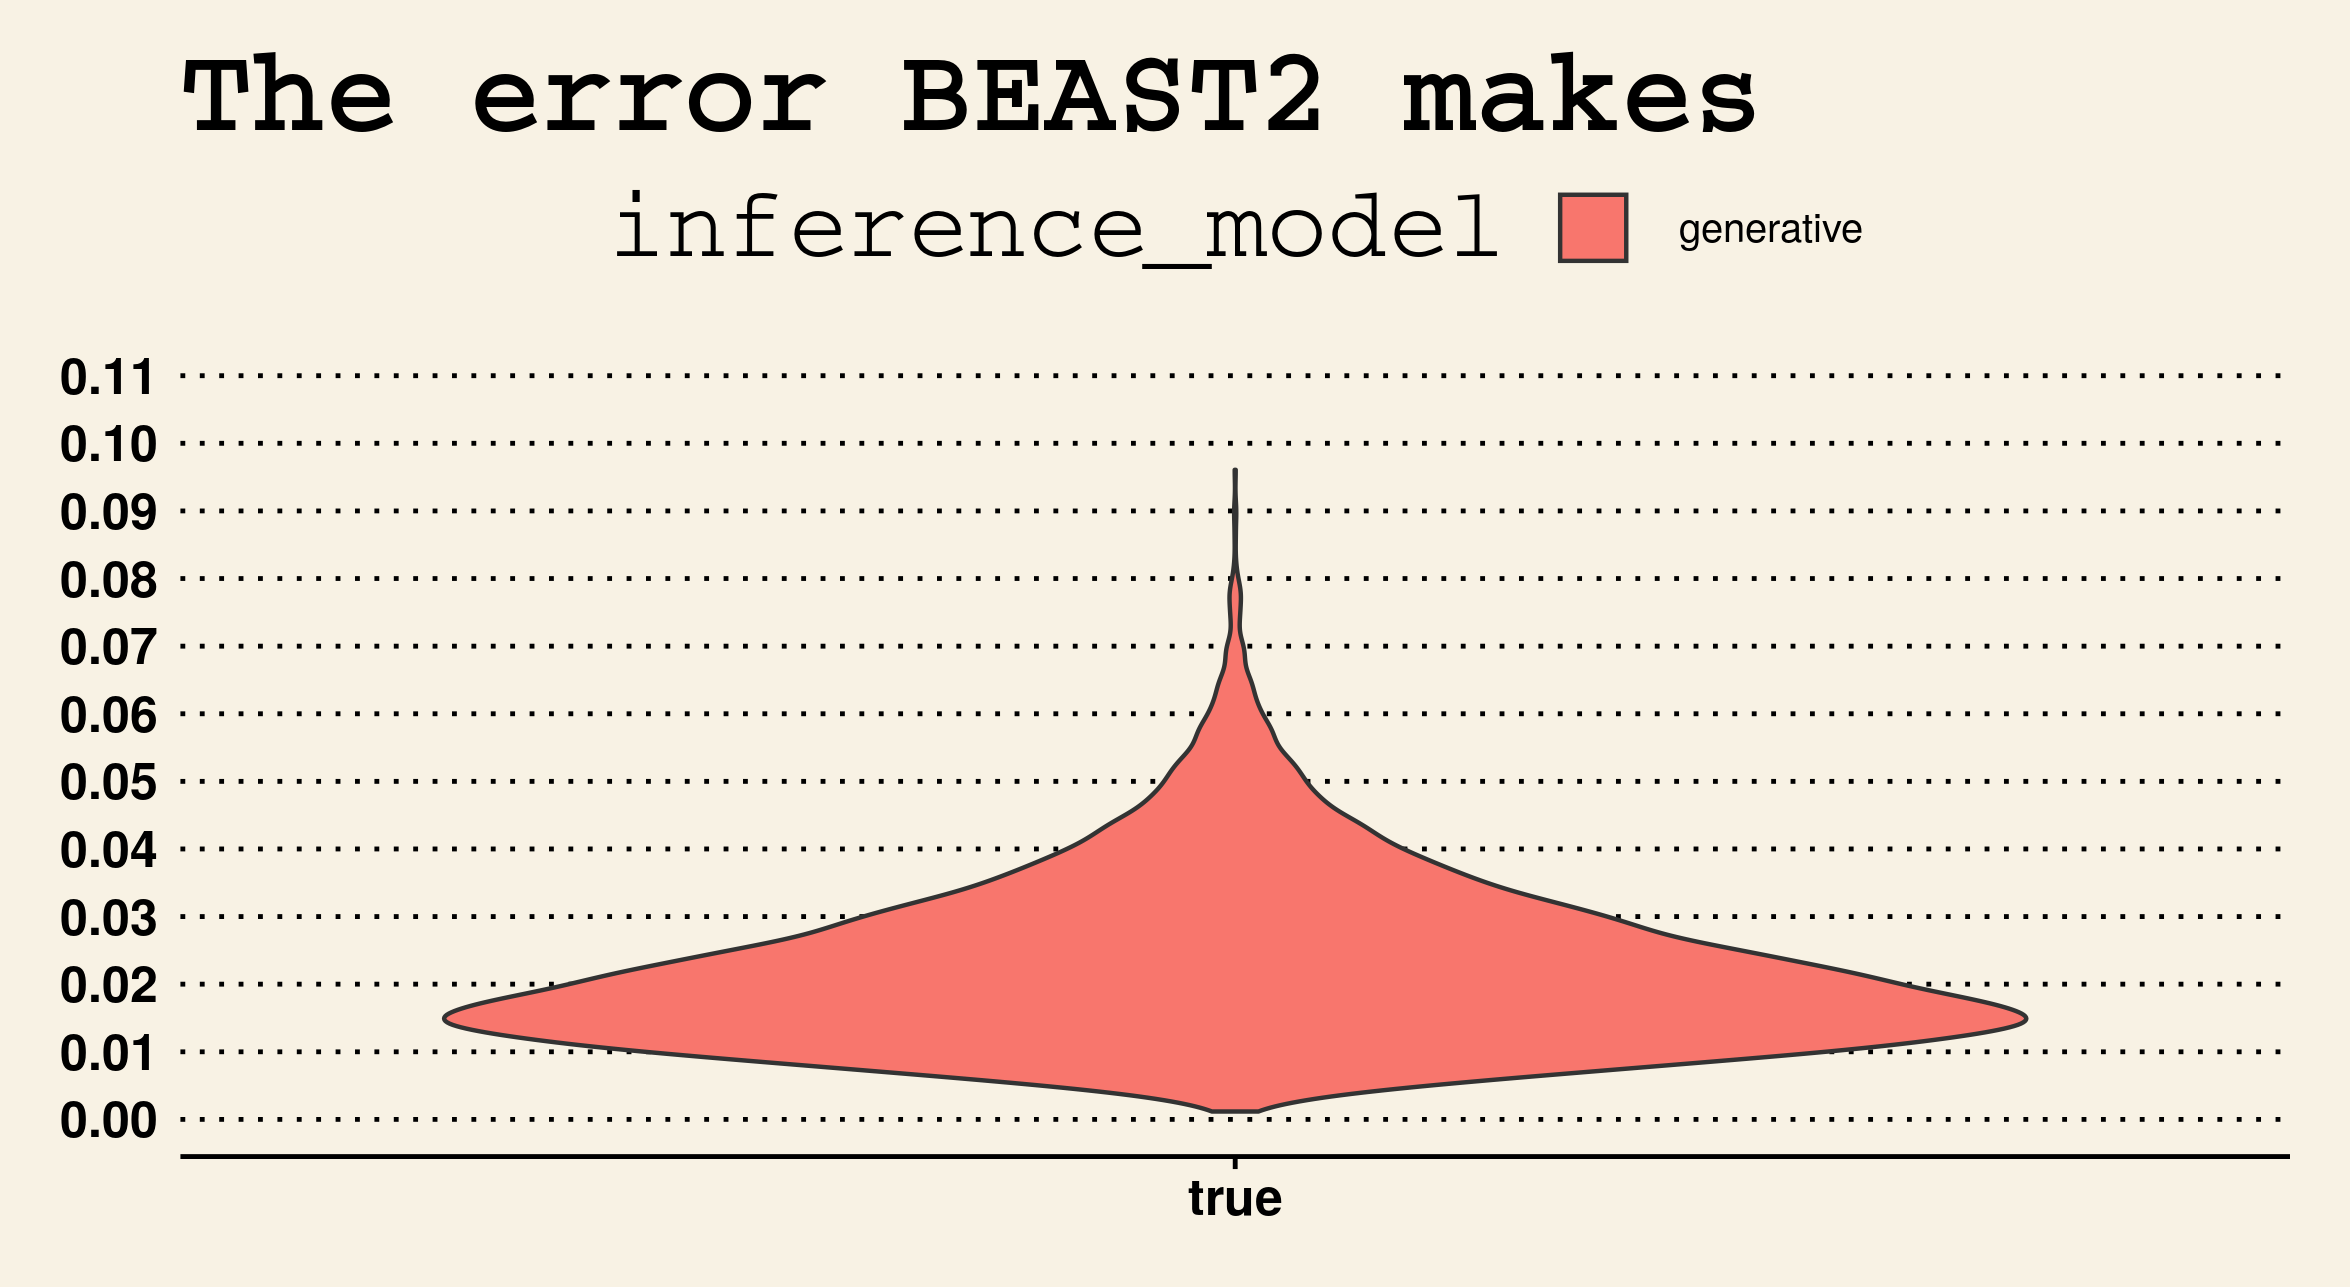
\includegraphics[width=\textwidth]{figure_example_1.png}
  \caption{
    Example 1: the error BEAST2 makes from a phylogeny 
    when the generative and inference model are the same.
  }
  \label{fig:example_1}
\end{figure}

The error distribution obtained in this way can serve as a control:
imagine one develops a novel tree prior related to the Yule model.
One can predict that BEAST2 will be worse in recovering the phylogenies
from that novel tree prior, as only the existing tree priors are used
in inference. 
To determine how much worse the recovery is, one needs to know the 
inference error made by existing tree priors. 
As this control is important, it is an inherent part of \verb;pirouette;:
it is called twinning, which is shown in example research question 3.

%%%%%%%%%%%%%%%%%%%%%%%%%%%%%%%%%%%%%%%%%%%%%%%%%%%%%%%%%%%%%%%%%%%%%%%%%%%%%%%%%%%%%%
\section{Usage: Example Research Question 2}
%%%%%%%%%%%%%%%%%%%%%%%%%%%%%%%%%%%%%%%%%%%%%%%%%%%%%%%%%%%%%%%%%%%%%%%%%%%%%%%%%%%%%%

A second research question that \verb;pirouette; can answer, is:

"What is the error made by BEAST2 from a phylogeny when
picking the best inference model?"

Here we start with a tree generated from an unknown 
diversification model, that has six taxa and a crown age of ten:

\begin{lstlisting}[
  language=R, 
  floatplacement=ht, 
  frame=single, 
  label = {lst:unknown_phylogeny},
  caption = A phylogeny generated by an unknown diversification model.
]
phylogeny  <- ape::read.tree(
  text = "(((A:8, B:8):1, C:9):1, ((D:8, E:8):1, F:9):1);"
)
\end{lstlisting}
\begin{figure}[ht]
  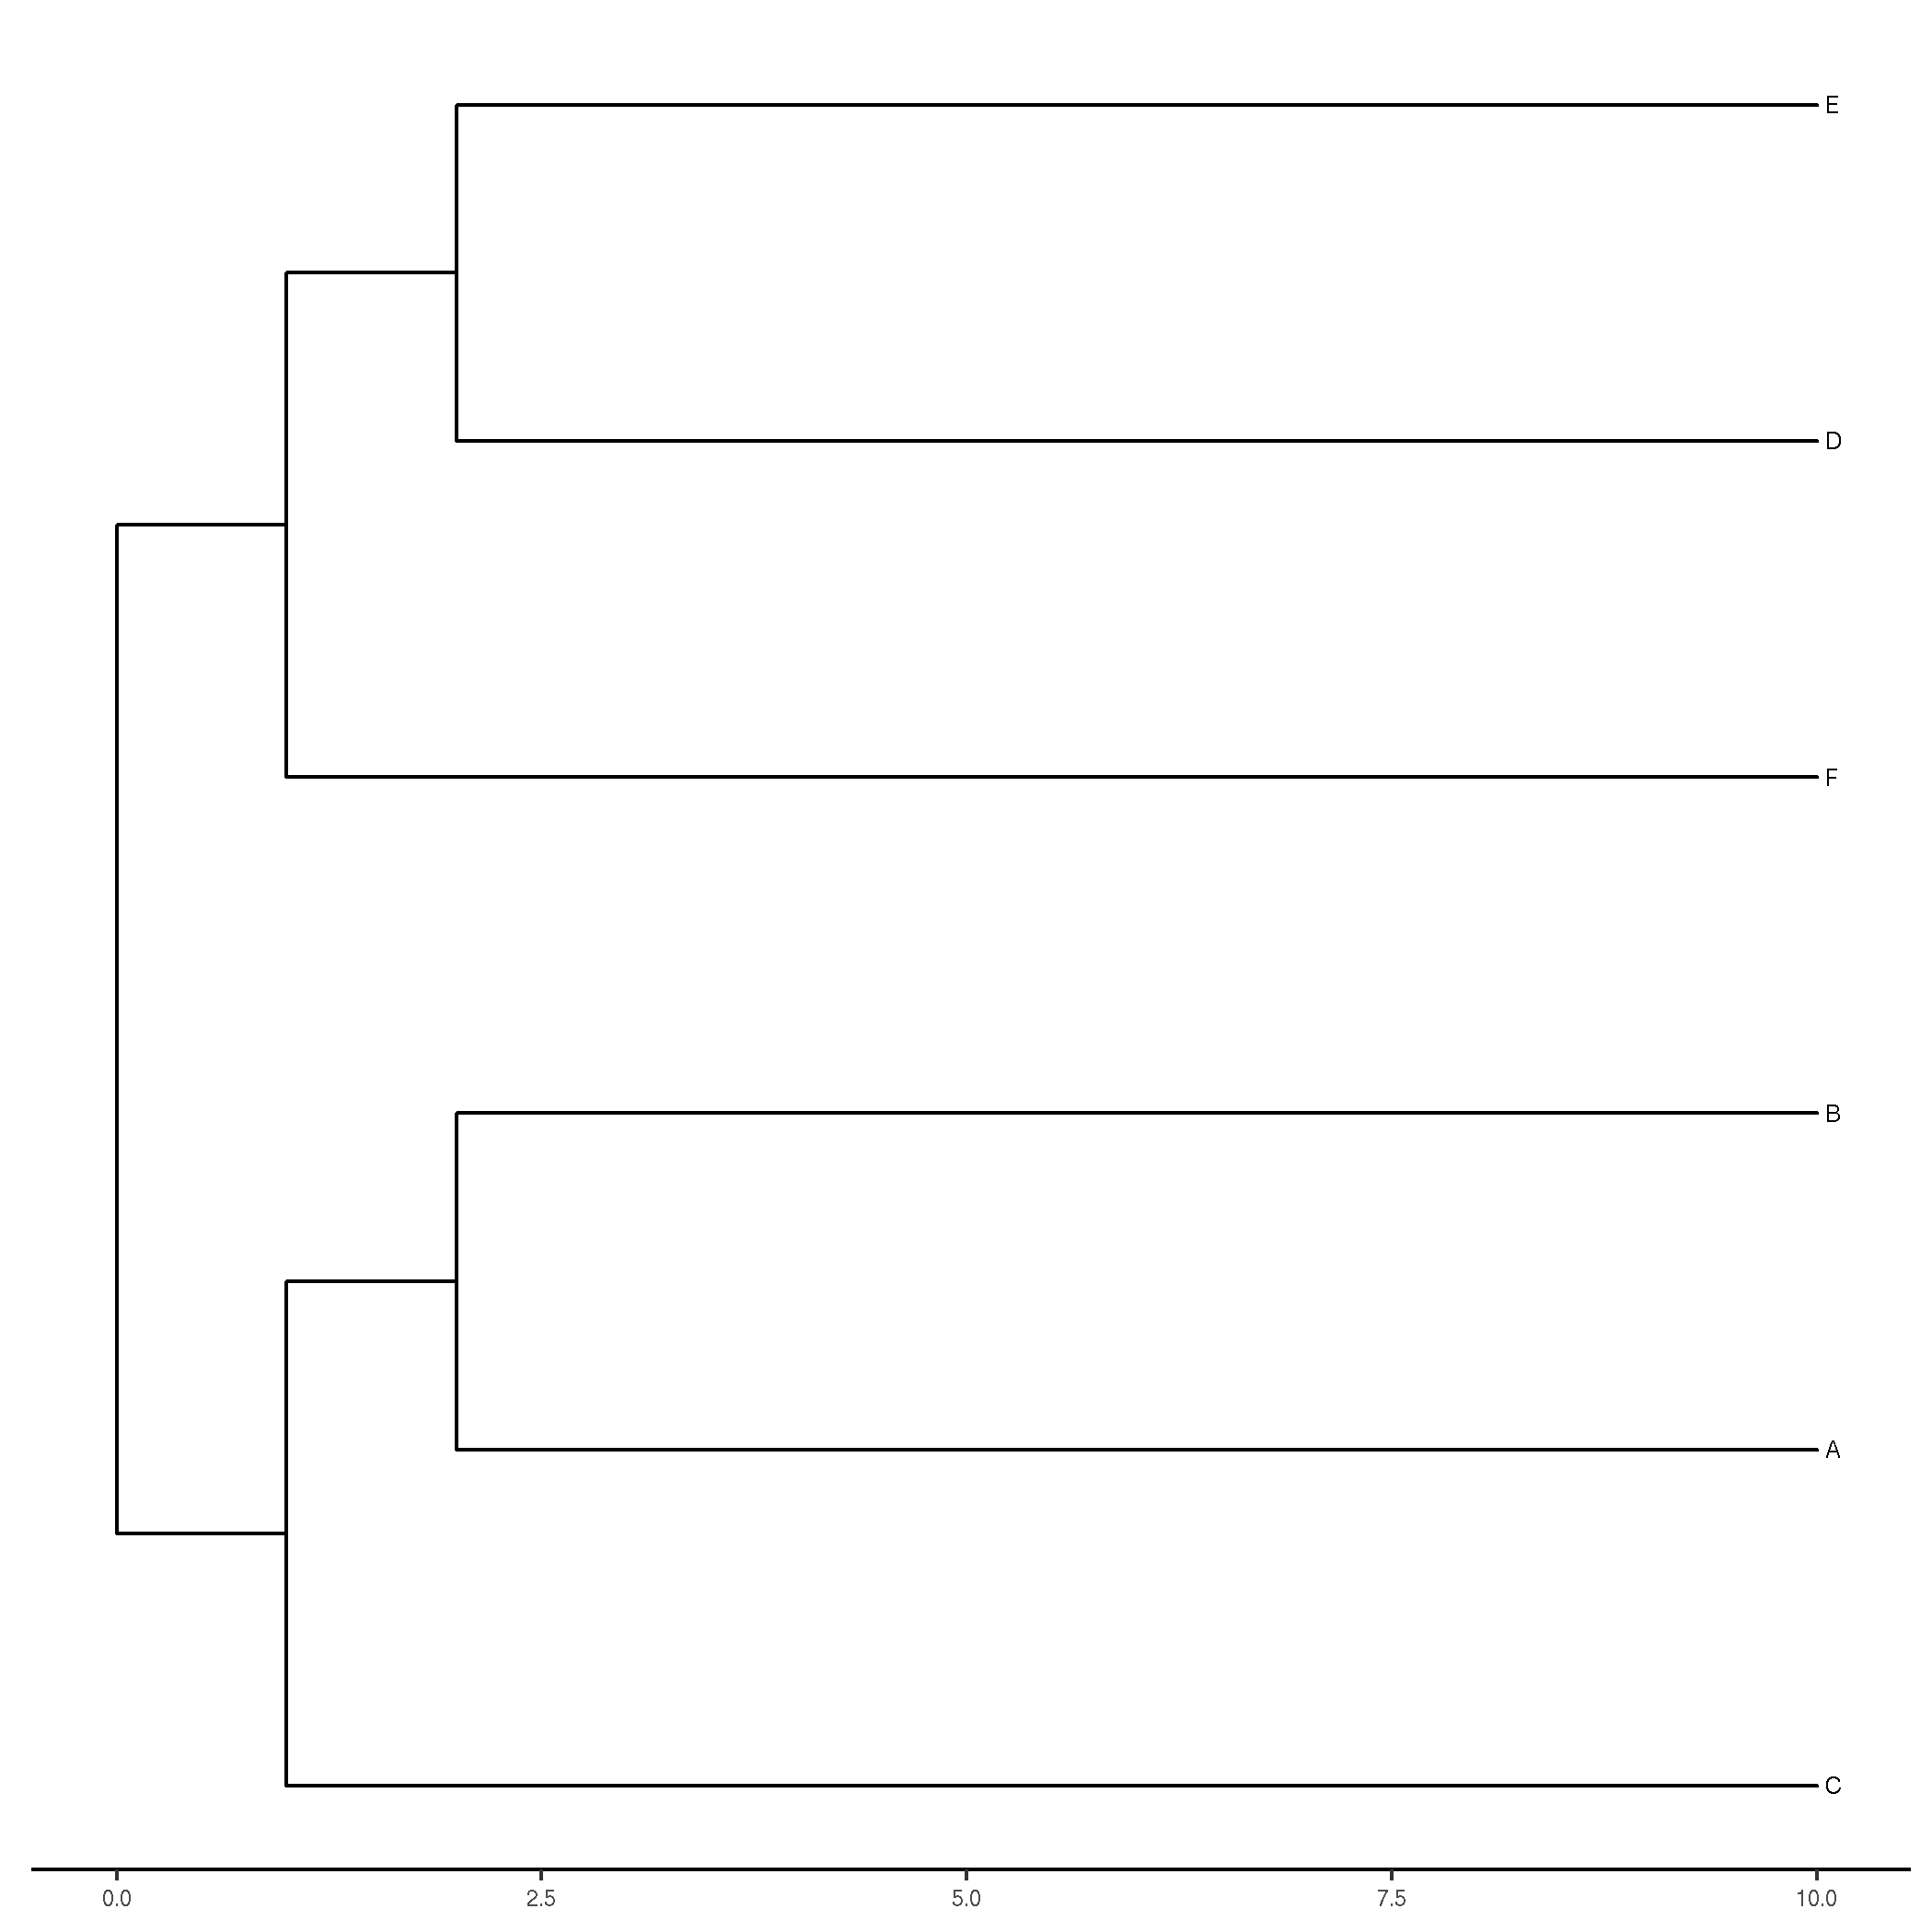
\includegraphics[width=\textwidth]{tree_unknown.png}
  \caption{The tree derived from an unknown diversification process, 
    as created by listing \ref{lst:unknown_phylogeny}.
  }
\end{figure}

The first step in \verb;pirouette; is to simulate a DNA alignment from the given phylogeny. 
We will re-use the alignment parameters of the previous example 
as shown in listing \ref{lst:create_alignment}.

\begin{table}
  \begin{tabular}{ | c | c | c | l | }
    \hline
    \textbf{model type} & \textbf{run if} & \textbf{measure evidence} & \textbf{inference model} \\ 
    \hline
    candidate & best candidate & yes & JC, strict, Yule \\
    candidate & best candidate & yes & JC, strict, BD   \\
    ...       & ...            & ... & ...              \\
    candidate & best candidate & yes & GTR, RLN, CCP    \\
    candidate & best candidate & yes & GTR, RLN, CEP    \\
    \hline
  \end{tabular}
  \caption{
    Experimental setup to answer the second research question.
    JC: Jukes-Cantor site model.
    strict: strict clock model.
    Yule: Yule (pure-birth) tree prior.
    BD: birth-death tree prior.
    GTR: GTR site model.
    RLN: relaxed log-normal clock model.
    CCP: coalescent constant-population tree prior.
    CEP: coalescent exponential-population tree prior.
  }
\end{table}

In the second step we state our experiments. 
Within this example, all our experiments are candidates,
run only if it is the best candidate, the evidence is measured (ignoring
this will give a helpful error) and we use the full set of 
40 inference models, which are all combinations of 4 site 
models, 2 clock models and 5 tree priors.

\begin{lstlisting}[
  language=R, 
  floatplacement=ht, 
  frame=single, 
  label = {lst:create_all_experiments},
  caption = Create all 40 candidate experiments
]
experiments <- create_all_experiments()
\end{lstlisting}

Also here, the third (the BEAST2 inference) and fourth (measuring the error)
steps have sensible defaults, and we are not
interested in using a twin tree. We can create the complete
\verb;pirouette; parameter set (again) like this:

\begin{lstlisting}[language=R, floatplacement=ht, frame=single]
pir_params <- create_pir_params(
  alignment_params = alignment_params,
  experiments = experiments
)
\end{lstlisting}

Running the experiment:

\begin{lstlisting}[language=R, floatplacement=ht, frame=single]
errors <- pir_run(
  phylogeny,
  pir_params = pir_params
)
\end{lstlisting}

Again, showing the results:

\begin{lstlisting}[language=R, floatplacement=ht, frame=single]
pir_plot(errors)
\end{lstlisting}

The resulting figure is shown in figure \ref{fig:example_2}.

\giovanni{describe winner}
\richel{agreed, after the figures also show it :-) }

\begin{figure}[ht]
  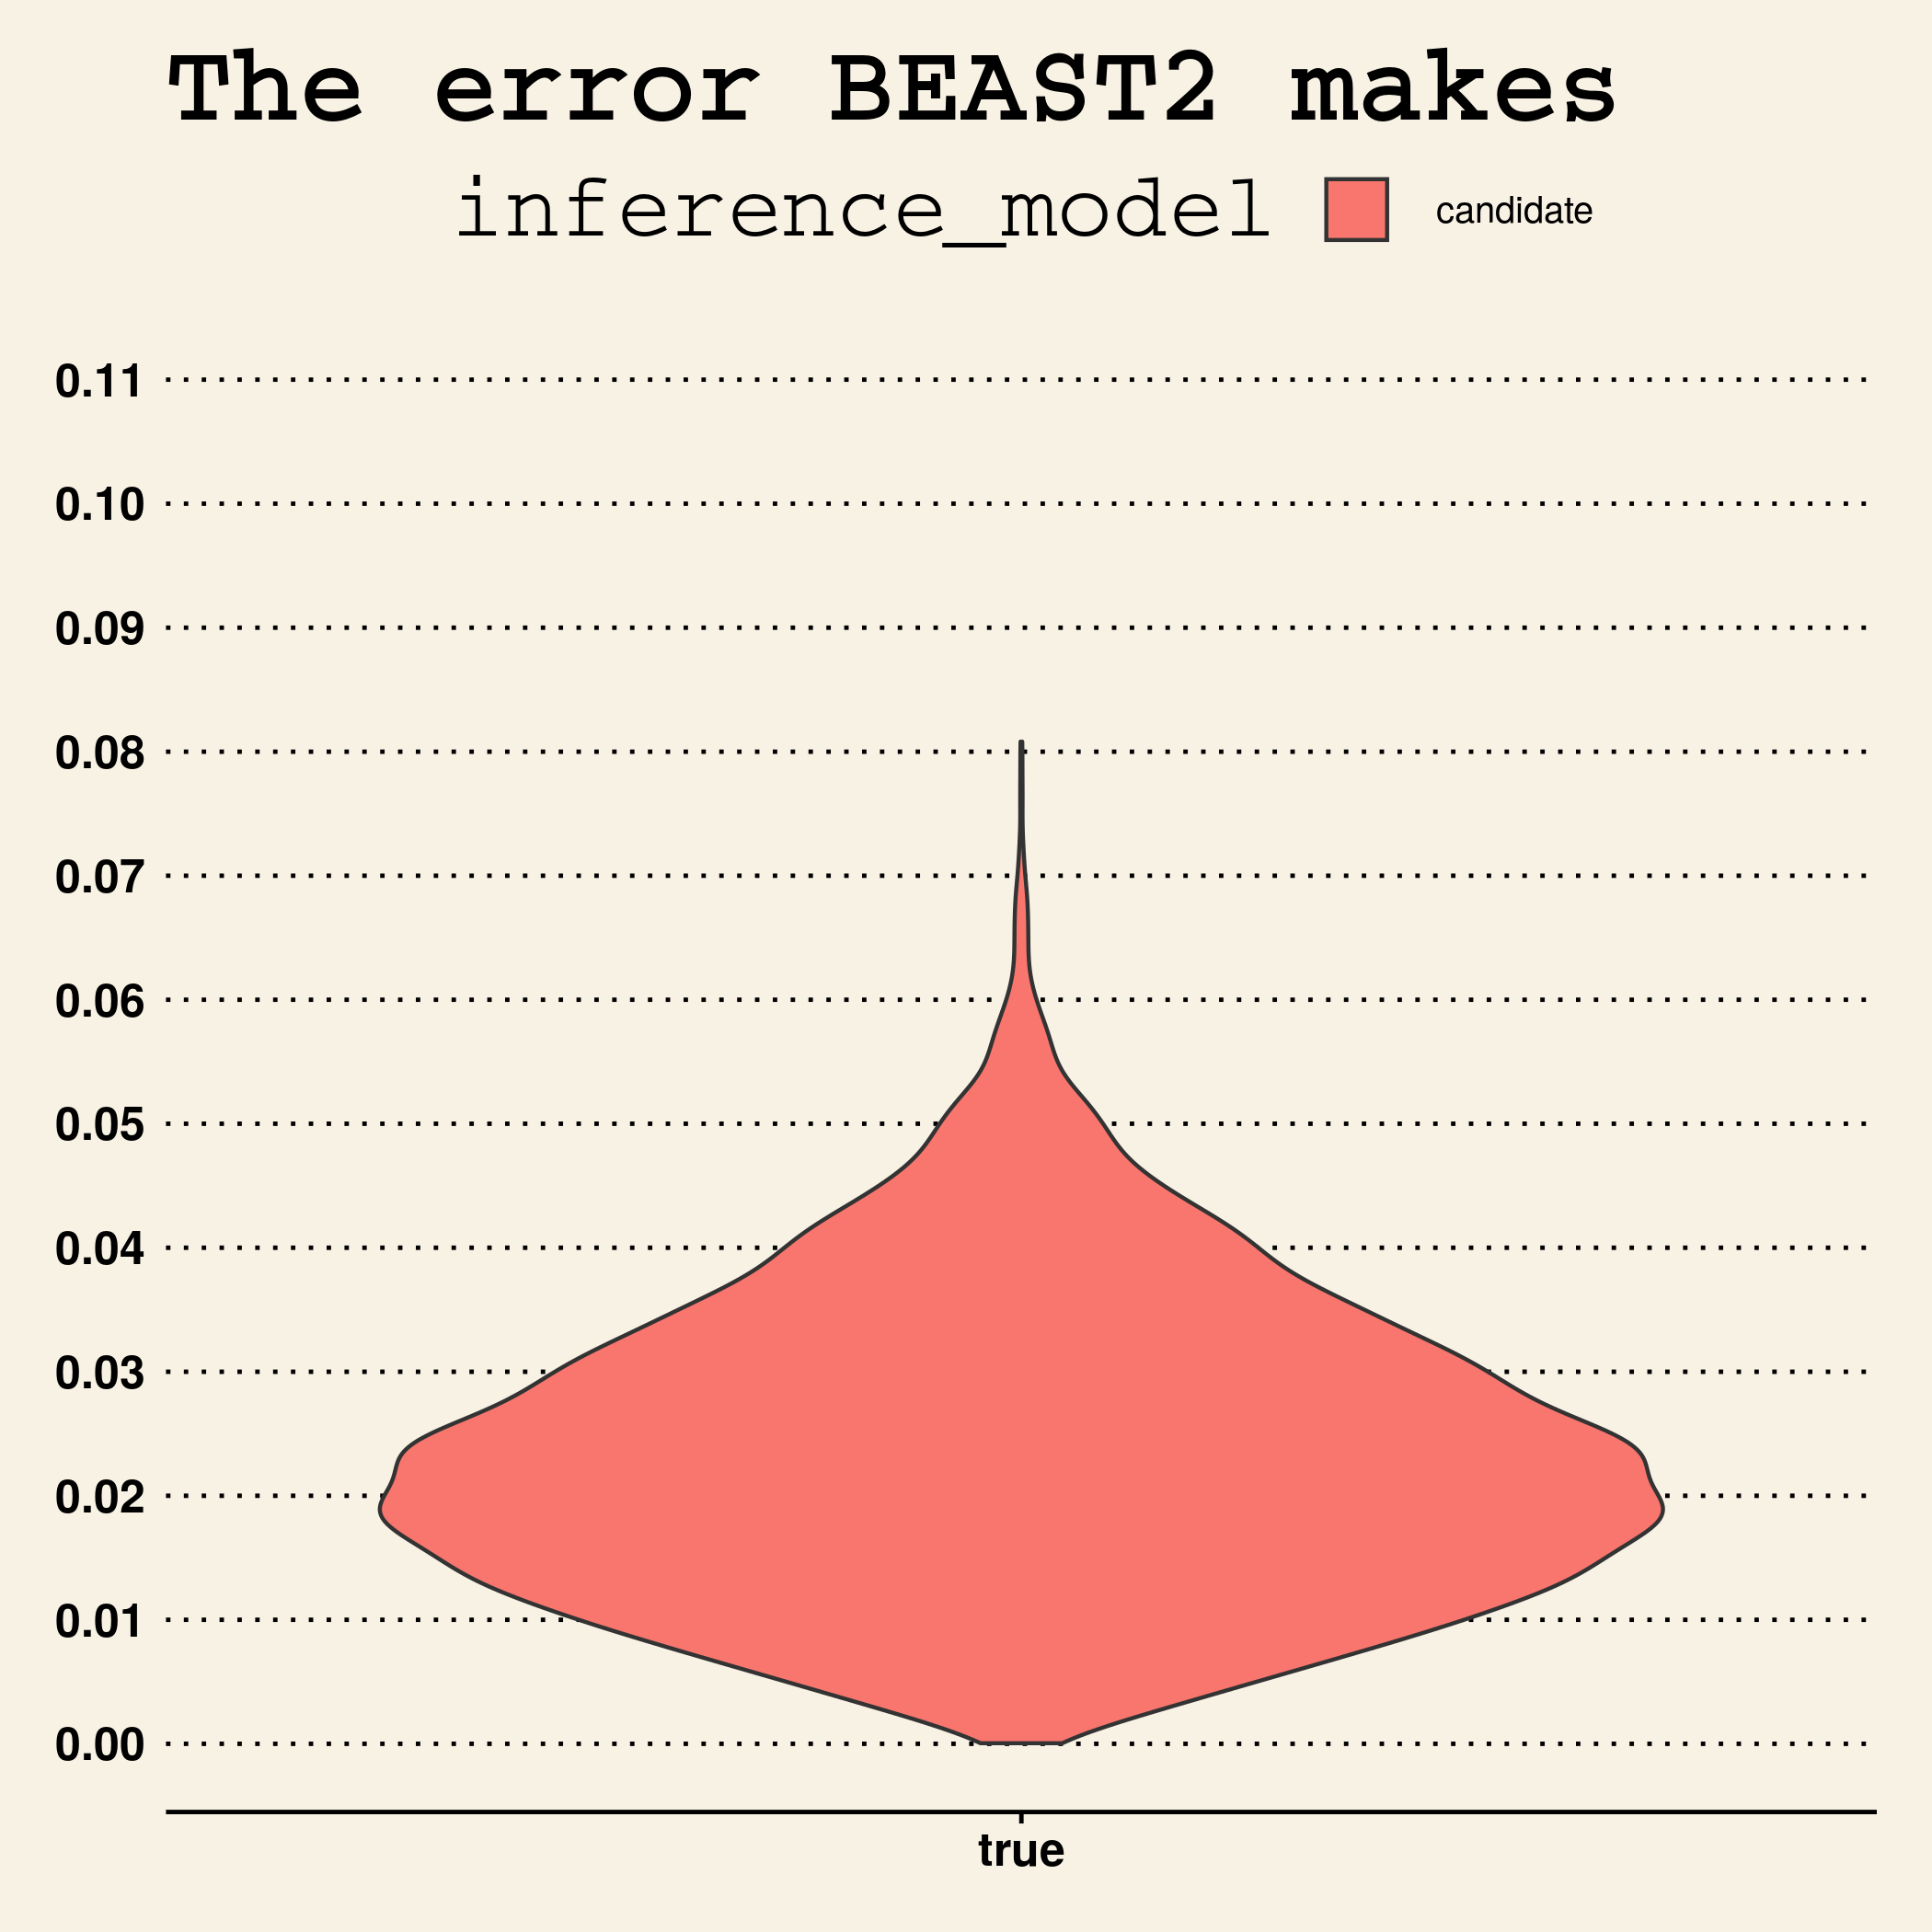
\includegraphics[width=\textwidth]{figure_example_2.png}
  \caption{
    Example 2: the error BEAST2 makes from a phylogeny when
    picking the best inference model.
    The x-axis specifies the tree type (which can be 'true' or 'twin'), 
    the y-axis shows the error
  }
  \label{fig:example_2}
\end{figure}

%%%%%%%%%%%%%%%%%%%%%%%%%%%%%%%%%%%%%%%%%%%%%%%%%%%%%%%%%%%%%%%%%%%%%%%%%%%%%%%%%%%%%%
\section{Usage: Example Research Question 3}
%%%%%%%%%%%%%%%%%%%%%%%%%%%%%%%%%%%%%%%%%%%%%%%%%%%%%%%%%%%%%%%%%%%%%%%%%%%%%%%%%%%%%%

A third research question that \verb;pirouette; can answer is:

"What is the error made by BEAST2 from a phylogeny, 
when hand-picking an inference model, compared to the background noise?"

Most of the settings for this example research question are
the same as in the previous section, which are
the phylogeny from an unknown speciation model (listing \ref{lst:unknown_phylogeny}), 
the alignment parameters (listing \ref{lst:create_alignment}) 
and the list of experiments (listing \ref{lst:create_generative_experiment}).

This time, however, we are interested in creating a twin tree,
as such a twin tree allows us to measure a baseline error produced
by the BEAST2 run.
A twin tree
has the same topology as the given tree, 
yet its branching times are simulated according 
to a tree prior already implemented by BEAST2 to produce a posterior. 
Because for a twin tree we know the tree prior 
and because we use that tree prior in inference, 
we expect BEAST2 to produce a posterior of phylogenies
that is close to the twin tree.
As the inference model for the twin tree is (more) completely
specified than the true tree, 
we expect that a twin tree and its posterior trees are more similar
than a true tree and its posterior trees.
Due to this, the twinning is used a control for the experiment.

Creating a twinning parameter is easy, as it has sensible default settings:

\begin{lstlisting}[
  language=R, 
  floatplacement=ht, 
  frame=single,
  label = {lst:create_twinning_params},
  caption = Create the default twinning parameters
]
twinning_params <- create_twinning_params()
\end{lstlisting}

We can now measure the errors made by BEAST2 
when inferring the given phylogeny 
versus the error it makes when the same procedure is applied to the twin tree.

All the \verb;pirouette; arguments are bundled and checked by \verb;create_pir_params;:

\begin{lstlisting}[language=R, floatplacement=ht, frame=single]
pir_params <- create_pir_params(
  alignment_params = alignment_params,
  experiments = experiments,
  twinning_params = twinning_params
)
\end{lstlisting}

Running:

\begin{lstlisting}[language=R, floatplacement=ht, frame=single]
errors <- pir_run(
  phylogeny,
  pir_params = pir_params
)
\end{lstlisting}

Again, showing the results:

\begin{lstlisting}[language=R, floatplacement=ht, frame=single]
pir_plot(errors)
\end{lstlisting}

The resulting figure is shown in figure \ref{fig:example_3}

\begin{figure}[ht]
  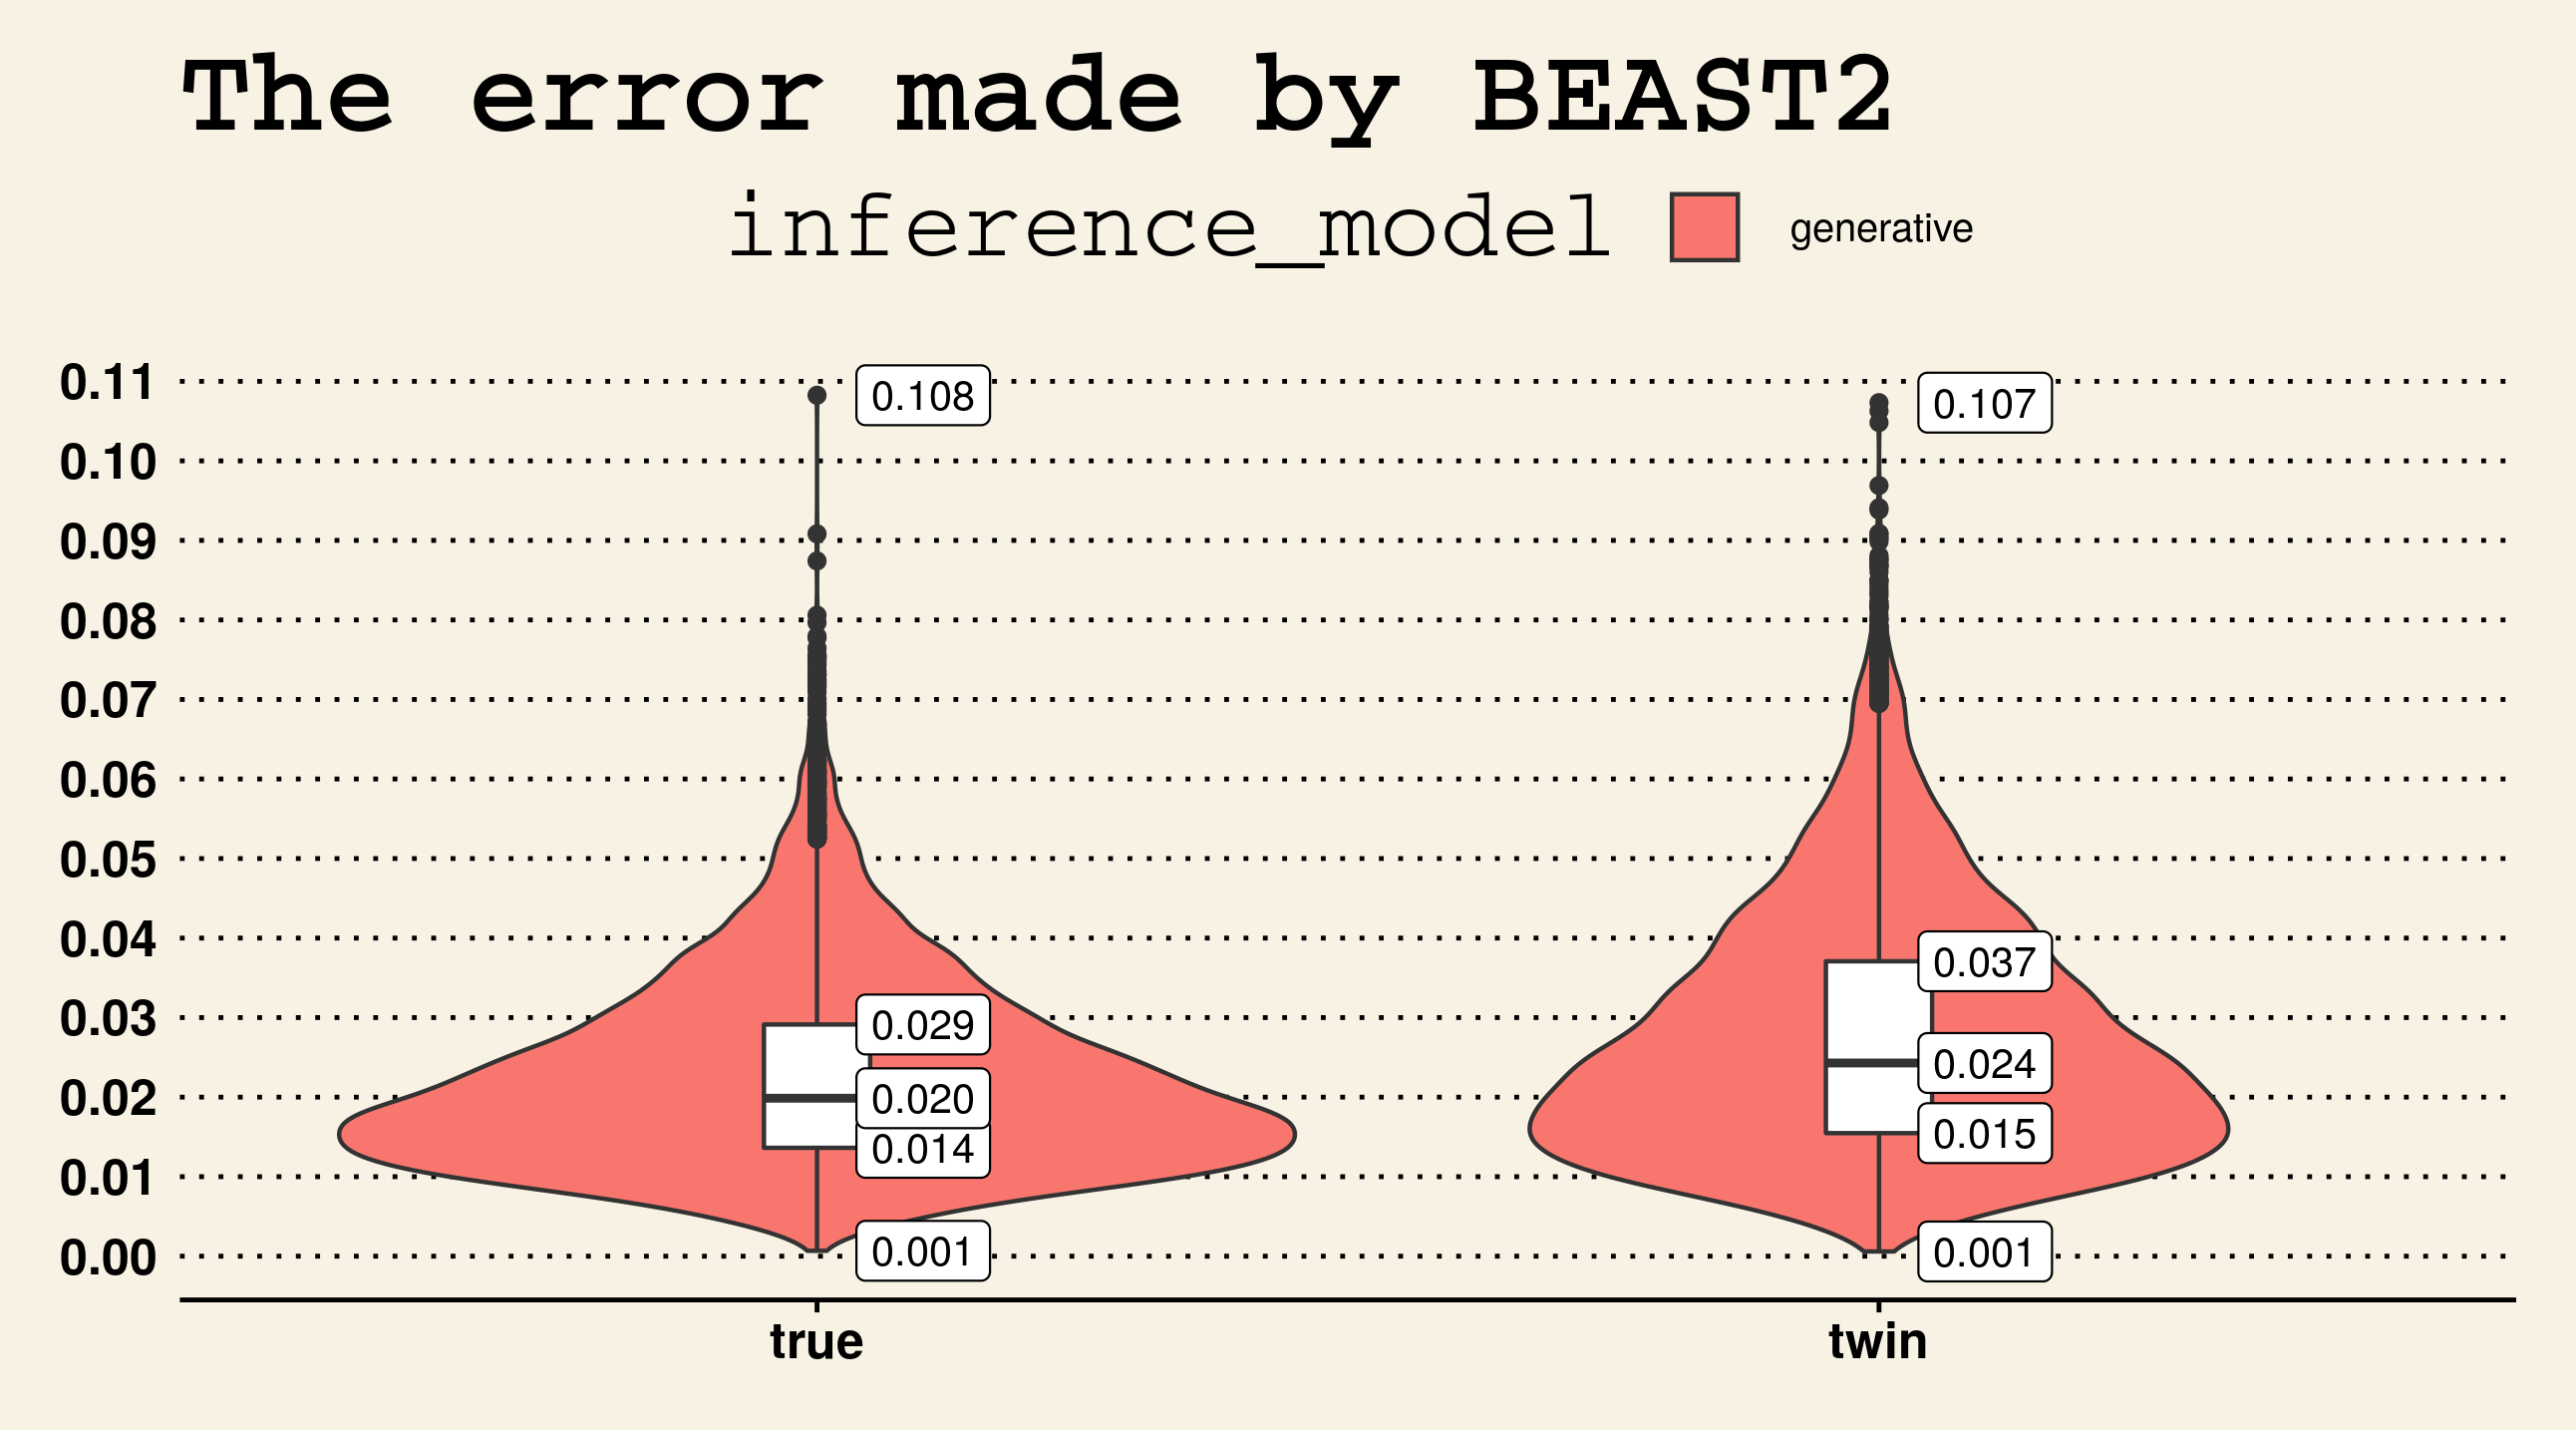
\includegraphics[width=\textwidth]{figure_example_3.png}
  \caption{
    Example 3: the error made by BEAST2 from a phylogeny, picking the best inference model versus the control.
    Here, the twin column shows the error BEAST2 makes starting from the original tree versus the twin. 
    The x-axis specifies the tree type (which can be 'true' or 'twin'), the y-axis shows the error.
    The boxplot shows the minimum, first quartile, median, third 
    quartile and maximum error, of which the values are displayed 
    in the adjacent label.
  }
  \label{fig:example_3}
  \giovanni{remove boxplots}
\end{figure}

\iffalse
The error BEAST2 makes from a phylogeny 
picking the best inference model, compared to the background noise.
Here, the twin column shows the error BEAST2 makes on an idealized
tree, to measure the noise, which is the minimal error. 
\fi


%%%%%%%%%%%%%%%%%%%%%%%%%%%%%%%%%%%%%%%%%%%%%%%%%%%%%%%%%%%%%%%%%%%%%%%%%%%%%%%%%%%%%%
\section{Usage: Example Research Question 4}
%%%%%%%%%%%%%%%%%%%%%%%%%%%%%%%%%%%%%%%%%%%%%%%%%%%%%%%%%%%%%%%%%%%%%%%%%%%%%%%%%%%%%%

A fourth research question that \verb;pirouette; can answer, is:

"What is the error made by BEAST2 from a phylogeny 
derived from an unknown speciation model,
when selecting the best inference model, 
in relationship to the background error?"
\richel{
  I inserted this example research question, 
  as think this is natural intermediate between the 
  previous and next/final example
}

Here, same as example 2 and 3, we start with the phylogeny 
from an unknown speciation model (listing \ref{lst:unknown_phylogeny}), 
The first step in \verb;pirouette; is to simulate a DNA alignment 
from the given phylogeny, for which we will use the same code 
as shown in listing \ref{lst:create_alignment}.

In the second step we specify we want all 
40 inference models to compete, by 
calling \verb;create_all_experiments;,
as done in listing \ref{lst:create_all_experiments}.

We choose again to use sensible defaults for the third (the BEAST2 inference) 
and fourth (measuring the error) steps, 
as we previously did to answer the second research question. 

To get an idea of a baseline error made by BEAST2, 
we also make use of the twinning option by using the
default created twinning parameters, as shown in 
listing \ref{lst:create_twinning_params}.

\begin{lstlisting}[language=R, floatplacement=ht, frame=single]
pir_params <- create_pir_params(
  alignment_params = alignment_params,
  experiments = experiments,
  twinning_params = twinning_params
)
\end{lstlisting}

Running the experiment:

\begin{lstlisting}[language=R, floatplacement=ht, frame=single]
errors <- pir_run(
  phylogeny,
  pir_params = pir_params
)
\end{lstlisting}

Again, showing the results:

\begin{lstlisting}[language=R, floatplacement=ht, frame=single]
pir_plot(errors)
\end{lstlisting}

The resulting figure is shown in figure \ref{fig:example_4}.

\giovanni{describe winner}
\richel{agreed, after the figures also show it :-) }

\begin{figure}[ht]
  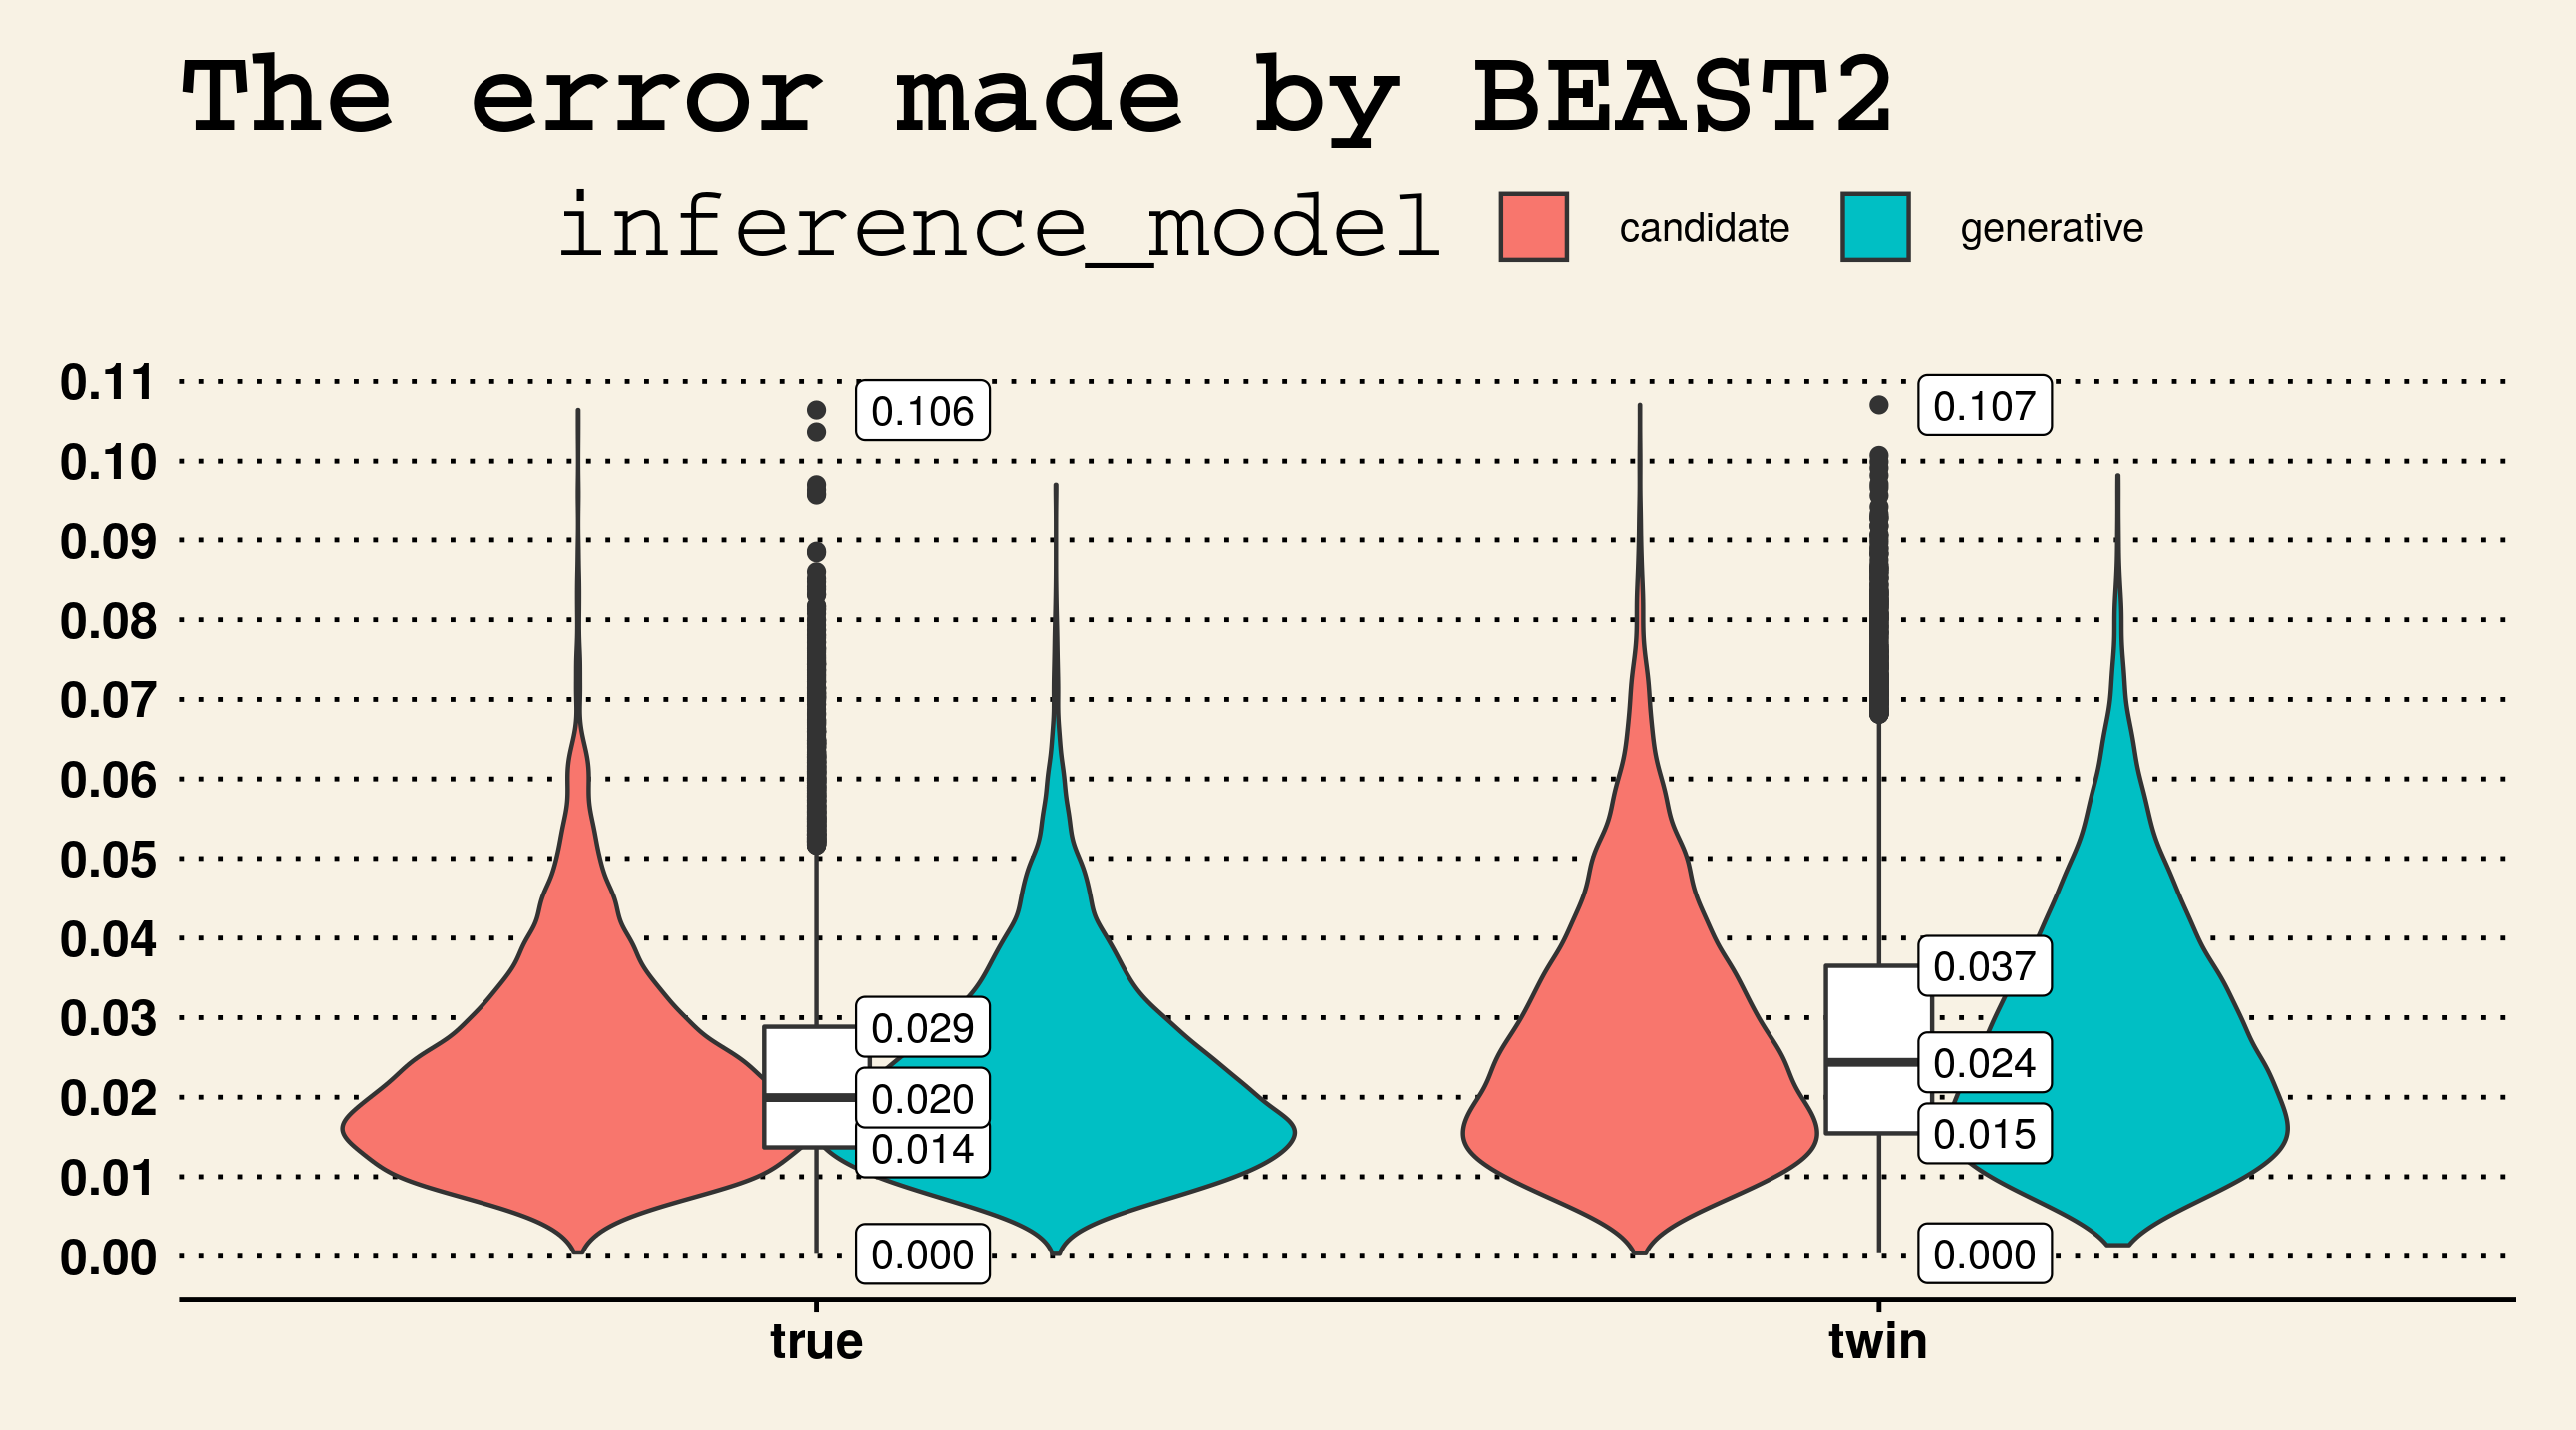
\includegraphics[width=\textwidth]{figure_example_4.png}
  \caption{
    Example 4: the error made by BEAST2 from a phylogeny, when the generative model is known, compared to candidates with similar inference models, in relationship to the background error.
    The x-axis specifies the tree type, the y-axis shows the error.
    The boxplot shows the minimum, first quartile, median, third 
    quartile and maximum error, of which the values are displayed 
    in the adjacent label.
  }
  \label{fig:example_4}
  \giovanni{Remove boxplots.}
\end{figure}


%%%%%%%%%%%%%%%%%%%%%%%%%%%%%%%%%%%%%%%%%%%%%%%%%%%%%%%%%%%%%%%%%%%%%%%%%%%%%%%%%%%%%%
\section{Usage: Example Research Question 5}
%%%%%%%%%%%%%%%%%%%%%%%%%%%%%%%%%%%%%%%%%%%%%%%%%%%%%%%%%%%%%%%%%%%%%%%%%%%%%%%%%%%%%%

A fifth research question that \verb;pirouette; can answer, is:

"What is the error made by BEAST2 from a phylogeny, 
when the generative model is known, 
compared to candidates with similar inference models, 
in relationship to the background error?"

In this example, we use a tree generated by the Yule process.
Instead of using the common Yule tree as in example 2, we'll use
a Yule tree of low (actually: zero) likelihood: 
the one as used in examples 3 and 4.
by using the code shown in listing \ref{lst:create_yule_tree}.
The first step in \verb;pirouette; is to simulate a DNA alignment 
from the given phylogeny, for which we will use the same code 
as shown in listing \ref{lst:create_alignment}.

\begin{table}
  \begin{tabular}{ | c | c | c | l | }
    \hline
    \textbf{model type} & \textbf{run if} & \textbf{measure evidence} & \textbf{inference model} \\ 
    \hline
    generative & always         & yes & JC, strict, Yule \\
    candidate  & best candidate & yes & JC, strict, BD \\
    candidate  & best candidate & yes & JC, strict, CCP \\
    candidate  & best candidate & yes & JC, strict, CEP \\
    \hline
  \end{tabular}
  \caption{
    Experimental setup to answer the fourth research question.
    JC: Jukes-Cantor site model.
    strict: strict clock model.
    Yule: Yule (pure-birth) tree prior.
    BD: birth-death tree prior.
    CCP: coalescent constant-population tree prior.
    CEP: coalescent exponential-population tree prior.
  }
  \label{tab:experiment_5}
\end{table}

In the second step we state our experiments. 
In this example, we must both specify the generative and candidate experiments. Here we specify the generative model:

\begin{lstlisting}[language=R, floatplacement=H, frame=single]
generative_experiment <- create_experiment(
  model_type = "generative",
  run_if = "always",
  do_measure_evidence = TRUE
)
\end{lstlisting}

Specifying all candidates can be done simply by calling \verb;create_all_experiments;. In this case, all candidates will use the same site and clock model, and only differ in their tree priors:

\begin{lstlisting}[language=R, floatplacement=H, frame=single]
candidate_experiments <- create_all_experiments(
  site_models = list(create_jc69_site_model()),
  clock_models = list(create_strict_clock_model()),
  tree_priors = list(
    create_bd_tree_prior(), 
    create_ccp_tree_prior(), 
    create_cep_tree_prior()
  )
)
\end{lstlisting}

We need to combine these experiments into one set:

\begin{lstlisting}[language=R, floatplacement=H, frame=single]
experiments <- c(list(generative_experiment), candidate_experiments)
\end{lstlisting}

We choose again to use sensible defaults for the third (the BEAST2 inference) and fourth (measuring the error) steps, as we previously did to answer the second research question. To get an idea of a baseline error made by BEAST2, we also make use of the twinning option:

\begin{lstlisting}[language=R, floatplacement=H, frame=single]
pir_params <- create_pir_params(
  alignment_params = alignment_params,
  experiments = experiments,
  twinning_params = create_twinning_params()
)
\end{lstlisting}

Running the experiment:

\begin{lstlisting}[language=R, floatplacement=H, frame=single]
errors <- pir_run(
  phylogeny,
  pir_params = pir_params
)
\end{lstlisting}

Again, showing the results:

\begin{lstlisting}[language=R, floatplacement=H, frame=single]
pir_plot(errors)
\end{lstlisting}

The resulting figure is shown in figure \ref{fig:example_5}.

\giovanni{describe winner}
\richel{agreed, after the figures also show it :-) }

\begin{figure}[h]
  
\includegraphics[width=\textwidth]{figure_example_5.png}
  \caption{
    Example 5: the error made by BEAST2 from a phylogeny, when the generative model is known, compared to candidates with similar inference models, in relationship to the background error.
    The x-axis specifies the tree type, the y-axis shows the error.
    The boxplot shows the minimum, first quartile, median, third 
    quartile and maximum error, of which the values are displayed 
    in the adjacent label
  }
  \label{fig:example_5}
\end{figure}

%%%%%%%%%%%%%%%%%%%%%%%%%%%%%%%%%%%%%%%%%%%%%%%%%%%%%%%%%%%%%%%%%%%%%%%%%%%%%%%%%%%%%%
\section{Discussion}
%%%%%%%%%%%%%%%%%%%%%%%%%%%%%%%%%%%%%%%%%%%%%%%%%%%%%%%%%%%%%%%%%%%%%%%%%%%%%%%%%%%%%%

In the four example research questions we showed how to use \verb;pirouette; 
to assess if BEAST2 is able, with a birth-death prior, 
to recover the original tree simulated by a Yule process. 
In principle any other, possibly much more complex, 
generative prior can be tested.
All tests were performed on a single original tree, 
hence not providing us enough statistical power to 
evaluate the level of accuracy of the inference. 

However if the same procedure were repeated and performed on a distribution 
with a sufficient number of generative trees, 
it could actually constitute a quantitative assessment 
of the quality of the inference.
To give an idea of the insights \verb;pirouette; can give,
we pretend the results of the example research questions
to be obtained from thousands of replicates.
In that case, figure \ref{fig:example_1} shows 
the minimum error BEAST2 when the
generative model is known, which can serve as 
a minimum noise level assessment in a bigger experiment.  
Figure \ref{fig:example_2} shows that 
\richel{
  reword after new results with 6 taxa tree
} 
the best candidate model gives an error distribution similar to the unknown tree prior,
hinting that the candidate model would be just as good in inference.
Figure \ref{fig:example_3} shows that 
\richel{
  reword after new results with 6 taxa tree
} 
the twin model gives an error distribution similar to the unknown tree prior,
hinting that the shape of the phylogeny with unknown tree prior
does not effect the error made by BEAST2.
Figure \ref{fig:example_4} shows that 
\richel{
  reword after new results with 6 taxa tree
} 
the twin model and best candidate model give 
an error distribution similar to the unknown tree prior,
hinting that the shape of the phylogeny with unknown tree prior
does not effect the error made by BEAST2, 
and that the candidate model would be just as good in inference.

In conclusion, \verb;pirouette; can directly show 
the comparison between the results obtained 
on a new generative prior as compared to the error BEAST2 
would make when operating on a tree generated 
under a known, right and existing tree prior (the twin tree).
From such results an user can estimate whether or not a new tree prior, 
tailored on the generative process, is needed. 
If this would indeed be the case, 
one could implement their own tree prior as a new module in BEAST2.

%%%%%%%%%%%%%%%%%%%%%%%%%%%%%%%%%%%%%%%%%%%%%%%%%%%%%%%%%%%%%%%%%%%%%%%%%%%%%%%%%%%%%%
\section{pirouette resources}
%%%%%%%%%%%%%%%%%%%%%%%%%%%%%%%%%%%%%%%%%%%%%%%%%%%%%%%%%%%%%%%%%%%%%%%%%%%%%%%%%%%%%%

\verb;pirouette; is free, libre and open source software available at 
\url{http://github.com/richelbilderbeek/pirouette}
and is licensed under the GNU General Public License v3.0.
\verb;pirouette; follows all practices as recommended by the
literature: continuous integration, a code coverage of 100\%
and a style guide (\cite{style_guide}).
\verb;pirouette; depends on multiple packages, which are 
\verb;ape; (\cite{APE}), 
\verb;babette; (\cite{bilderbeek2018babette}),
\verb;ggplot2; (\cite{ggplot2}),
\verb;knitr; (\cite{knitr}),
\verb;mcbette; (\cite{mcbette}),
\verb;phangorn; (\cite{phangorn}),
\verb;rmarkdown; (\cite{rmarkdown}),
\verb;stringr; (\cite{stringr}),
\verb;testit; (\cite{testit}) and 
\verb;usethis; (\cite{usethis}).

\verb;pirouette;'s development takes place on GitHub,
\url{https://github.com/richelbilderbeek/pirouette}, 
which facilitates feature requests and 
has guidelines on how to do so.

\verb;pirouette;'s documentation is extensive. 
All functions are documented in the package's internal documentation. 
For quick use, 
each exported function shows a minimal example. 
For easy exploration, each exported function's documentation links to related functions.
Additionally, \verb;pirouette; has a vignette that demonstrates extensively how to use it. 

%%%%%%%%%%%%%%%%%%%%%%%%%%%%%%%%%%%%%%%%%%%%%%%%%%%%%%%%%%%%%%%%%%%%%%%%%%%%%%%%%%%%%%
\section{Citation of pirouette}
%%%%%%%%%%%%%%%%%%%%%%%%%%%%%%%%%%%%%%%%%%%%%%%%%%%%%%%%%%%%%%%%%%%%%%%%%%%%%%%%%%%%%%

Scientists using \verb;pirouette; in a published paper can cite this
article, and/or cite the \verb;pirouette; package 
directly. To obtain this citation from within an R script, use:

\begin{lstlisting}[language=R]
> citation("pirouette")
\end{lstlisting}

%%%%%%%%%%%%%%%%%%%%%%%%%%%%%%%%%%%%%%%%%%%%%%%%%%%%%%%%%%%%%%%%%%%%%%%%%%%%%%%%%%%%%%
\section{Acknowledgements}
%%%%%%%%%%%%%%%%%%%%%%%%%%%%%%%%%%%%%%%%%%%%%%%%%%%%%%%%%%%%%%%%%%%%%%%%%%%%%%%%%%%%%%

We would like to thank the Center for Information Technology of the University 
of Groningen for their support and for providing access to the Peregrine 
high performance computing cluster. 
We thank the Netherlands 
Organization for Scientific Research (NWO) for financial support 
through a VICI grant awarded to RSE.

%%%%%%%%%%%%%%%%%%%%%%%%%%%%%%%%%%%%%%%%%%%%%%%%%%%%%%%%%%%%%%%%%%%%%%%%%%%%%%%%%%%%%%
\section{Data Accessibility}
%%%%%%%%%%%%%%%%%%%%%%%%%%%%%%%%%%%%%%%%%%%%%%%%%%%%%%%%%%%%%%%%%%%%%%%%%%%%%%%%%%%%%%

All code is archived at \url{http://github.com/richelbilderbeek/pirouette_article},
with DOI \url{https://doi.org/12.3456/zenodo.1234567}.

%%%%%%%%%%%%%%%%%%%%%%%%%%%%%%%%%%%%%%%%%%%%%%%%%%%%%%%%%%%%%%%%%%%%%%%%%%%%%%%%%%%%%%
\section{Authors' contributions}
%%%%%%%%%%%%%%%%%%%%%%%%%%%%%%%%%%%%%%%%%%%%%%%%%%%%%%%%%%%%%%%%%%%%%%%%%%%%%%%%%%%%%%

RJCB, GL and RSE conceived the idea for the package. 
RJCB created and tested the package, and wrote the first draft of the manuscript.
GL tested the package and contributed substantially to revisions.
RSE contributed to revisions.

%%%%%%%%%%%%%%%%%%%%%%%%%%%%%%%%%%%%%%%%%%%%%%%%%%%%%%%%%%%%%%%%%%%%%%%%%%%%%%%%%%%%%%
% Bibliography
%%%%%%%%%%%%%%%%%%%%%%%%%%%%%%%%%%%%%%%%%%%%%%%%%%%%%%%%%%%%%%%%%%%%%%%%%%%%%%%%%%%%%%
% MEE style
\bibliographystyle{mee}
\bibliography{article}
%%%%%%%%%%%%%%%%%%%%%%%%%%%%%%%%%%%%%%%%%%%%%%%%%%%%%%%%%%%%%%%%%%%%%%%%%%%%%%%%%%%%%%

\appendix

%%%%%%%%%%%%%%%%%%%%%%%%%%%%%%%%%%%%%%%%%%%%%%%%%%%%%%%%%%%%%%%%%%%%%%%%%%%%%%%%%%%%%%
\section{Results in detail}
%%%%%%%%%%%%%%%%%%%%%%%%%%%%%%%%%%%%%%%%%%%%%%%%%%%%%%%%%%%%%%%%%%%%%%%%%%%%%%%%%%%%%%

%%%%%%%%%%%%%%%%%%%%%%%%%%%%%%%%%%%%%%%%%%%%%%%%%%%%%%%%%%%%%%%%%%%%%%%%%%%%%%%%%%%%%%
\subsection{Errors}
%%%%%%%%%%%%%%%%%%%%%%%%%%%%%%%%%%%%%%%%%%%%%%%%%%%%%%%%%%%%%%%%%%%%%%%%%%%%%%%%%%%%%%

%%%%%%%%%%%%%%%%%%%%%%%%%%%%%%%%%%%%%%%%%%%%%%%%%%%%%%%%%%%%%%%%%%%%%%%%%%%%%%%%%%%%%%
\begin{table}[h]
\centering
\begin{tabular}{ | r | l | l | l | l | }
\hline
\multirow{2}{*}{\textbf{Example}} & \multicolumn{2}{c|}{\textbf{True tree}} 
                                  & \multicolumn{2}{c|}{\textbf{Twin tree}} \\
\cline{2-5}
                                  & \textbf{median} & \textbf{range} & \textbf{median} & \textbf{range} \\
\hline
1  & $0.02$  & $0.0 - 0.27$  &         &               \\
2  & $0.02$  & $0.0 - 0.08$  &         &               \\
3  & $0.018$ & $0.0 - 0.1$   & $0.019$ & $0.0 - 0.11$  \\
4C & $0.22$  & $0.0 - 0.088$ & $0.009$ & $0.0 - 0.056$ \\
4G & $0.020$ & $0.0 - 0.075$ & $0.013$ & $0.0 - 0.052$ \\
\hline
\end{tabular}
\caption{
  \richel{redo}
  Results of the examples. 
  For the true and twin tree,
  the median and range (1st and 3rd quartile) of the errors 
  is shown. Experiment 4 is split in two rows
  by either the candidate ('C') or generative model ('G')
}
\label{tab:results}
\end{table}
%%%%%%%%%%%%%%%%%%%%%%%%%%%%%%%%%%%%%%%%%%%%%%%%%%%%%%%%%%%%%%%%%%%%%%%%%%%%%%%%%%%%%%

%%%%%%%%%%%%%%%%%%%%%%%%%%%%%%%%%%%%%%%%%%%%%%%%%%%%%%%%%%%%%%%%%%%%%%%%%%%%%%%%%%%%%%
\subsection{Example 1}
%%%%%%%%%%%%%%%%%%%%%%%%%%%%%%%%%%%%%%%%%%%%%%%%%%%%%%%%%%%%%%%%%%%%%%%%%%%%%%%%%%%%%%

%%%%%%%%%%%%%%%%%%%%%%%%%%%%%%%%%%%%%%%%%%%%%%%%%%%%%%%%%%%%%%%%%%%%%%%%%%%%%%%%%%%%%%
\begin{figure}[h]
  \centering
  \resizebox {0.8\columnwidth} {!} {
    \begin{tikzpicture}[
      ->,>=stealth',shorten >=1pt,auto,
      node distance=0.25\textheight, 
      semithick
    ]   
    \tikzstyle{every state}=[]
    \node[state, draw=none] (O) [] {
    };   
    \node[state] (A) [right of = O, rectangle] {
      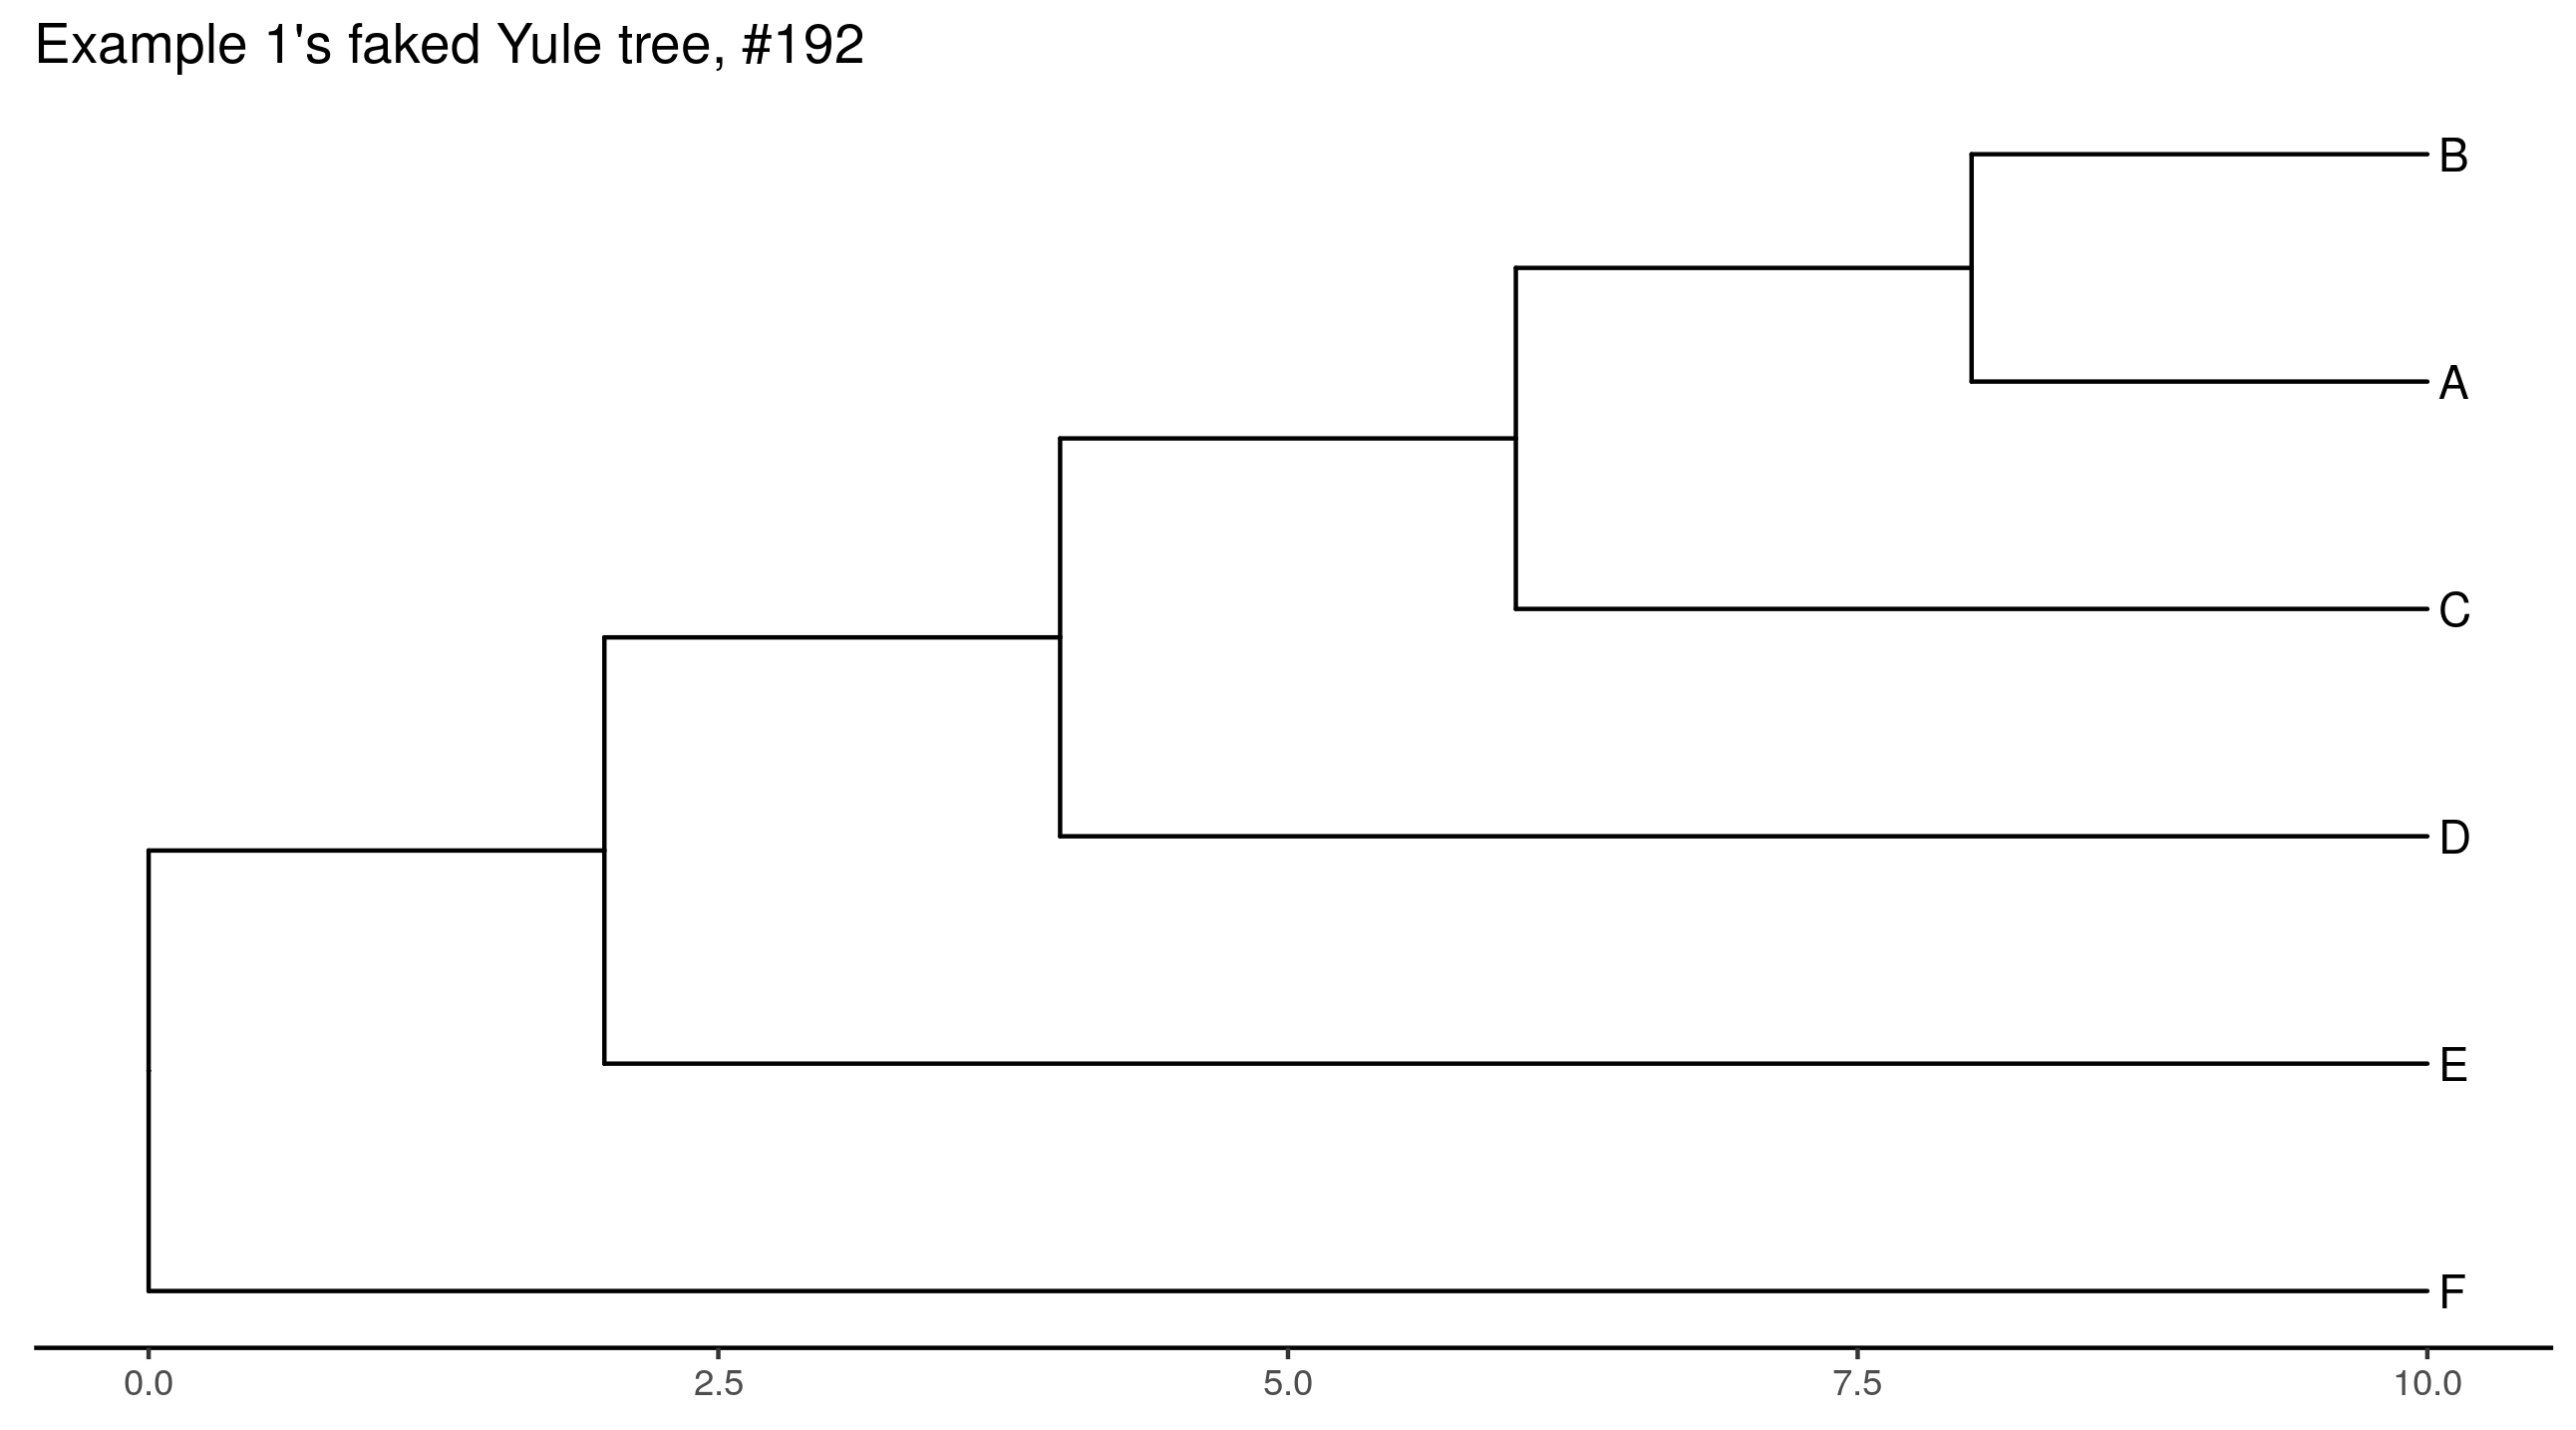
\includegraphics[height=0.2\textheight]{example_1_true_tree.png}
    };   
    \node[state] (B) [below of = A, rectangle] {
      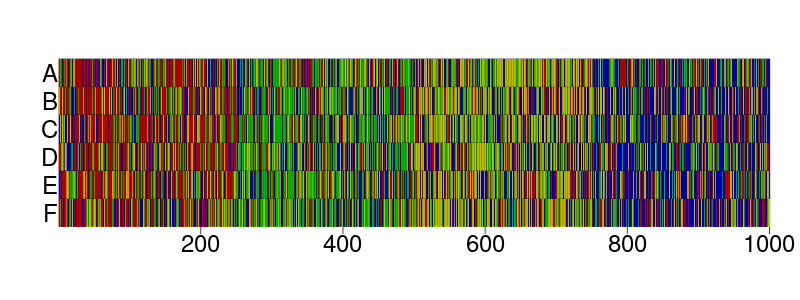
\includegraphics[height=0.2\textheight]{example_1_true_alignment.png}
    };   
    \node[state] (C) [below of = B, rectangle] {
      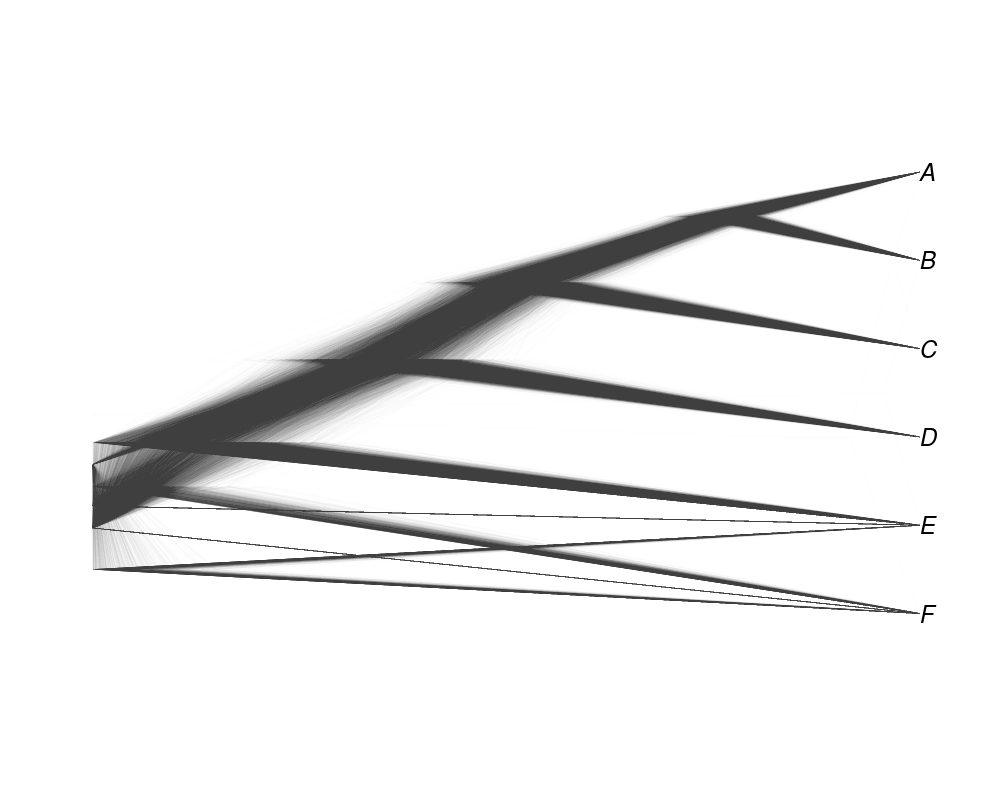
\includegraphics[height=0.2\textheight]{example_1_true_posterior_gen.png}
    };   
    \node[state] (D) [below of = C, rectangle] {
      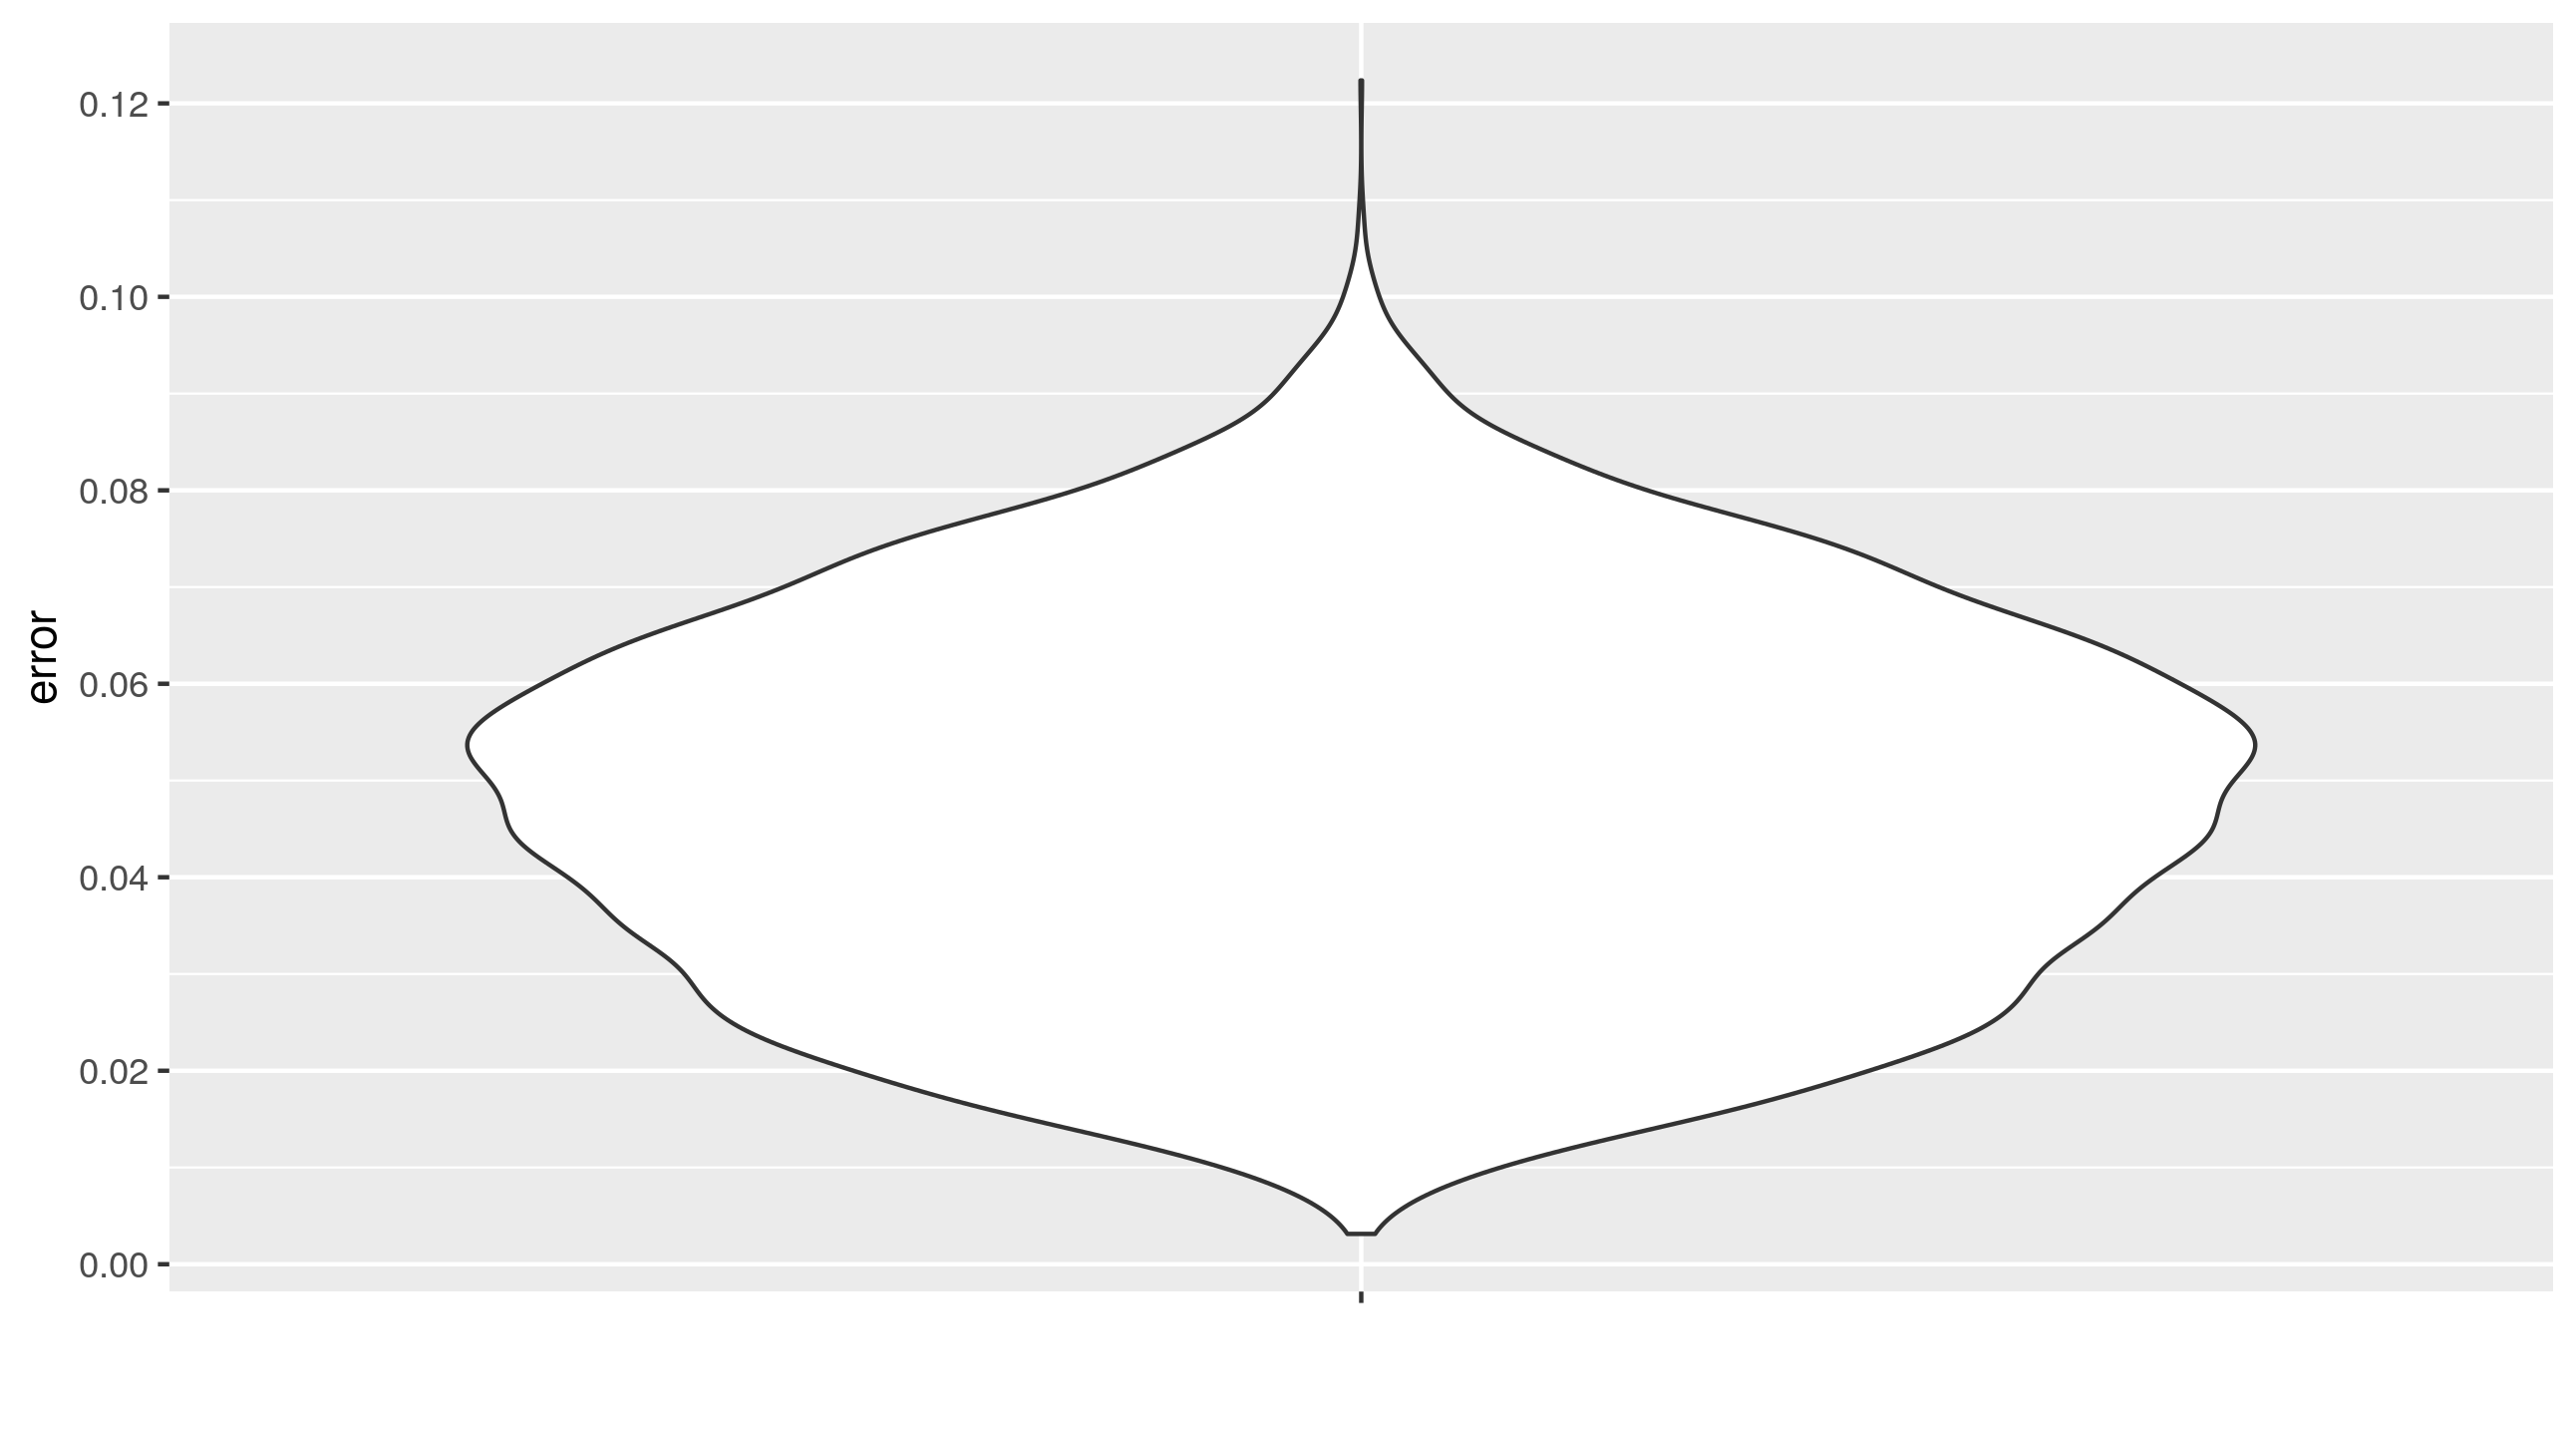
\includegraphics[height=0.2\textheight]{example_1_error_violin.png}
    };   
    \path 
      (O) edge [anchor = south] node {} (A)
      (A) edge [anchor = south] node {} (B)
      (B) edge [anchor = south] node {} (C)
      (C) edge [anchor = south] node {} (D)
    ; 
    \end{tikzpicture}
  }
\end{figure}
%%%%%%%%%%%%%%%%%%%%%%%%%%%%%%%%%%%%%%%%%%%%%%%%%%%%%%%%%%%%%%%%%%%%%%%%%%%%%%%%

%%%%%%%%%%%%%%%%%%%%%%%%%%%%%%%%%%%%%%%%%%%%%%%%%%%%%%%%%%%%%%%%%%%%%%%%%%%%%%%%%%%%%%

\input{example_1_esses.latex}
% has label tab:esses_example_1

%%%%%%%%%%%%%%%%%%%%%%%%%%%%%%%%%%%%%%%%%%%%%%%%%%%%%%%%%%%%%%%%%%%%%%%%%%%%%%%%%%%%%%
\subsection{Example 2}
%%%%%%%%%%%%%%%%%%%%%%%%%%%%%%%%%%%%%%%%%%%%%%%%%%%%%%%%%%%%%%%%%%%%%%%%%%%%%%%%%%%%%%

\input{example_2_esses.latex}
% has label tab:esses_example_2

\input{example_2_evidences.latex}
% has label tab:evidences_example_2

%%%%%%%%%%%%%%%%%%%%%%%%%%%%%%%%%%%%%%%%%%%%%%%%%%%%%%%%%%%%%%%%%%%%%%%%%%%%%%%%%%%%%%
\subsection{Example 3}
%%%%%%%%%%%%%%%%%%%%%%%%%%%%%%%%%%%%%%%%%%%%%%%%%%%%%%%%%%%%%%%%%%%%%%%%%%%%%%%%%%%%%%

\input{example_3_esses.latex}
% has label tab:esses_example_3

%%%%%%%%%%%%%%%%%%%%%%%%%%%%%%%%%%%%%%%%%%%%%%%%%%%%%%%%%%%%%%%%%%%%%%%%%%%%%%%%%%%%%%
\subsection{Example 4}
%%%%%%%%%%%%%%%%%%%%%%%%%%%%%%%%%%%%%%%%%%%%%%%%%%%%%%%%%%%%%%%%%%%%%%%%%%%%%%%%%%%%%%

\input{example_4_esses.latex}
% has label tab:esses_example_4

\input{example_4_evidences.latex}
% has label tab:evidences_example_4

\end{document}
